\chapter{Truth Discovery (old)}
\label{chapter_td}

% \section{Introduction}
% \label{td_sec_introduction}

There is an increasing amount of data available in today's world, particularly
from the web, social media platforms and crowdsourcing systems. The openness of
such platforms makes it simple for a wide range of users to share information
quickly and easily, potentially reaching a wide international audience. It is
inevitable that amongst this abundance of data there are \emph{conflicts},
where data sources disagree on the truth regarding a particular object or
entity. For example, low-quality sources may mistakenly provide erroneous data
for topics on which they lack expertise.

Resolving such conflicts and determining the true facts is therefore an
important task. Truth discovery has emerged as a set of techniques to achieve
this by considering the \emph{trustworthiness} of
sources~\cite{li_survey_2016,gupta2011survey,berti2015veracity}. The general principle is that
true facts are those claimed by trustworthy sources, and trustworthy sources
are those that claim believable facts. Application areas include real-time
traffic navigation~\cite{du2019}, drug side-effect discovery~\cite{ma2017},
crowdsourcing and social
sensing~\cite{zhang_robust_2016,wang_truth_2012,ma_faitcrowd_2015}.

% Areas TD is already used include:
% \begin{itemize}
% \item Amazon wants the correct copyright information (https://www.nytimes.com/2019/08/19/technology/amazon-orwell-1984.html?smid=nytcore-ios-share)

% \item Facebook wants to rank sources by trust

% \item Drug side effects~\cite{ma2017}

% \item Facebook editor\footnote{\url{https://facebook.com/editor}} uses
% crowdsourcing by allowing users to suggest edits to pages to correct
% information or add new information (e.g.  coffee shop opening times).
% Contributor experience and reliability can be used to improve confidence in
% claims.~\cite{eisenschlos}

% \item Real-time traffic levels can be estimated by mobile crowdsourcing
%~\cite{aslam2012}, but varying data quality can present challenges (e.g. due to
% inaccurate sensors, issues with GPS in urban environments~\cite{gil2017}).
% Truth discovery approaches tailored specifically to mobile crowd sourcing have
% been developed.~\cite{du2019}

% \end{itemize}

\begin{figure}[b]
\centering
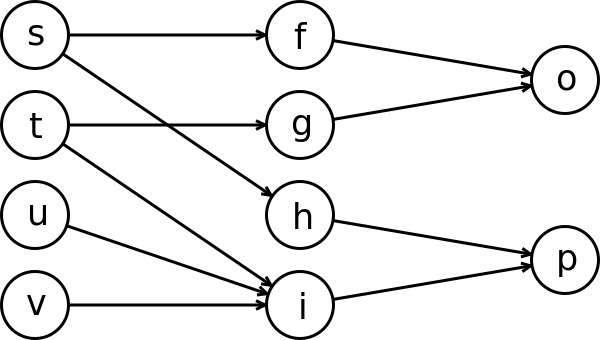
\includegraphics[scale=0.25]{intro_example}
\caption{
    Illustrative example of a dataset to which truth discovery can be applied
    with data sources $\{s, t, u, v\}$, facts $\{f, g, h, i\}$ and objects
    $\{o, p\}$
}
\label{td_fig_intro_example}
\end{figure}

For a simple example of a situation where trust can play an important role in
conflict resolution, consider the following example.

\begin{example}
\label{ex:intro_example}

Let $o$ and $p$ represent two images for which crowdsourcing workers are asked
to provide labels (in the truth discovery terminology, $o$ and $p$ are called
\emph{objects}). Consider workers (the data sources) $s, t, u$ and $v$ who put
forward potential labels $f, g$ for $o$, and $h, i$ for $p$, as shown in
\cref{td_fig_intro_example}; such potential answers are termed \emph{facts}. In the
graphical representation, sources, facts and objects are shown from left to
right, and the edges indicate claims made by sources and the objects to which
facts relate.

Without considering trust information, the label for $o$ appears a tie, with
both options $f$ and $g$ receiving one vote from sources $s$ and $t$
respectively.

Taking a trust-aware approach, however, we can look beyond object $o$ to
consider the \emph{trustworthiness} of $s$ and $t$. Indeed, when it comes to
object $p$, $t$ agrees with two extra sources $u$ and $v$, whereas $s$
disagrees with everyone. In principle there could be \emph{hundreds} of extra
sources here instead of just two, in which case the effect would be even more
striking. We may conclude that $s$ is \emph{less trustworthy} than $t$.
Returning to $o$, we see that $g$ is supported by a more trustworthy source,
and conclude that it should be accepted over $f$.

\end{example}

Many truth discovery algorithms have been proposed in the literature with a
wide range of techniques used, e.g. iterative heuristic-based
methods~\cite{pasternack2010,galland2010}, probabilistic models~\cite{yin2008},
maximum likelihood estimation and optimisation-based methods~\cite{li2016}, and
neural network
models~\cite{kotonya2020explainable,marshall2017neural,wang2018eann}. It is
common for such algorithms to be evaluated empirically by running them against
real-world or synthetic datasets for which the true facts are already known;
this allows \emph{accuracy} and other metrics to be calculated, and permits
comparison between algorithms (see \cite{waguih2014truth} for a systematic
empirical evaluation of this kind). This may be accompanied by some theoretical
analysis, such as calculating run-time complexity~\cite{gupta2011survey},
proving convergence of an iterative algorithm~\cite{yin_supervised_2011}, or
proving convergence to the `true' facts under certain assumptions on the
distribution of source
trustworthiness~\cite{xiao2016,xiao_thesis2018,ghosh_2011}.

A limitation of this kind of analysis is that the results only apply narrowly
to particular algorithms, due to the assumptions made (for instance, that
claims from sources follow a particular probability distribution). Such
assumptions can be problematic in domains where the desired truth is somewhat
`fuzzy'; for example, image classification problems and determining the
copyright status of
books.\footnote{\url{https://www.nytimes.com/2019/08/19/technology/amazon-orwell-1984.html}}

In this work we take first steps towards a more general approach, in which we
aim to study truth discovery
without reference to any specific methodology or probabilistic framework. To do
so we note the similarities between truth discovery and problems such as
judgment aggregation~\cite{endriss2016ja}, voting
theory~\cite{zwicker2016voting} ranking and recommendation
systems~\cite{altman2008,altman2005ranking,andersen2008,tennenholtz2004} in
which the \emph{axiomatic approach} of social choice has been successfully
applied.
%
In taking the axiomatic approach one aims to formulate \emph{axioms} that
encode intuitively desirable properties that an algorithm may possess. The
interaction between these axioms can then be studied; typical results include
\emph{impossibility results}, where it is shown that a set of axioms cannot
hold simultaneously, and \emph{characterisation results}, where it is shown
that a set of axioms are uniquely satisfied by a particular algorithm.

Such analysis brings a new \emph{normative} perspective to the truth discovery
literature. This complements empirical evaluation: in addition to seeing how well
an algorithm performs in practise on test datasets, one can check how well it
does against theoretical properties that any `reasonable' algorithm should
satisfy. The satisfaction (or failure) of such properties then shines new light
on the \emph{intuitive behaviour} of an algorithm, and may guide development of
new ones.

With this in mind, we develop a simplified framework for truth discovery in which
axioms can be formulated, and go on to give both an impossibility result and an
axiomatic characterisation of a baseline voting algorithm. We also analyse the
class of \emph{recursive} truth discovery algorithms, which includes many
existing examples from the literature. In particular, we analyse the well-known
algorithm \sums{}~\cite{pasternack2010} with respect to the axioms.

However, as a first step towards a social choice perspective of truth
discovery, our framework involves a number of simplifying assumptions not
commonly made in the truth discovery literature.

\begin{itemize}

    \item \textbf{Manipulation and collusion.} Some of our axioms assume
          sources are not \emph{manipulative}: they provide claims in good
          faith, and do not aim to misinform or artificially improve their
          standing with respect to the truth discovery algorithm. We also
          assume sources act independently, i.e. they do not \emph{collude}
          with or \emph{copy} one another.

    \item \textbf{Object correlations.} We do not model correlations between
          the objects of interest in the truth discovery problem. For example,
          in a crowdsourcing setting it may be known in advance that two
          objects $o$ and $p$ are similar, so that the true labels for
          $o$ and $p$ are correlated; this cannot be expressed in our
          framework.

    \item \textbf{Ordinal outputs.} For the most part, the outputs of our truth
          discovery methods consist of \emph{rankings} of the sources and
          facts. Thus, we describe when a source is considered \emph{more
          trustworthy} than another, but do not assign precise numerical values
          representing trustworthiness. This breaks with tradition in the truth
          discovery literature, but is a common point of view in social choice
          theory.

\end{itemize}

At first glance these are strong assumptions, and rule out potential
applications of our version of truth discovery. However, we argue that the
problem is non-trivial even in this simplified setting, and that interesting
axioms can still be put forth. The framework as set out here lays the
groundwork for these assumptions to be lifted in future work.

\begin{chapteroutline}
    Our framework is introduced and formally defined in
    \cref{td_sec_framework}. \Cref{td_sec_specific_operators} provides examples
    of truth discovery algorithms from the literature expressed in the
    framework. In \cref{td_sec_axioms} we formally introduce the axioms and
    present an impossibility result showing a subset of these cannot all be
    satisfied simultaneously. The examples of \cref{td_sec_specific_operators}
    are then revisited in \cref{td_sec_satisfaction_of_axioms}, where we
    analyse them with respect to the axioms and propose modifications to
    resolve some axiom failures. In \cref{td_sec_variable_domain} we extend the
    framework to allow variable domains of sources, facts and objects, and give
    an impossibility result similar to that of \cref{td_sec_axioms}. We discuss
    the axioms in \cref{td_sec_discussion} and related work in
    \cref{td_sec_relatedwork}. We conclude in \cref{td_sec_conclusion}. Missing
    proofs are given in \cref{chapter_td_proofs}.
\end{chapteroutline}

\section{An idealised framework for truth discovery}
\label{td_sec_framework}

In this section we define our formal framework, which provides the key
definitions required for theoretical discussion and analysis of truth discovery
methods.

For most of the chapter, we consider a fixed domain of finite and mutually
disjoint sets $\S$, $\F$ and $\O$ throughout, called the \emph{sources},
\emph{facts} and \emph{objects} respectively. All definitions and axioms will
be stated with respect to these sets.\footnote{We generalise to variable
domains in \cref{td_sec_variable_domain}.}

\subsection{Truth discovery networks}

A core definition of the framework is that of a \emph{truth discovery network},
which represents the input to a truth discovery problem. We model this as a
tripartite graph with certain constraints on its structure, in keeping with
approaches taken throughout the truth discovery
literature~\cite{yin2008,gupta2011survey}.

\begin{definition}
\label{def_td_network}
A \emph{truth discovery network} (hereafter a {\em TD network}) is a directed
graph $N = (V, E)$ where $V = \S \cup \F \cup \O$, and $E \subseteq (\S \times
\F) \cup (\F \times \O)$ has the following properties:

\begin{enumerate}
\item For each $f \in \F$ there is a unique $o \in \O$ with $(f, o) \in
E$, denoted $\obj_N(f)$. That is, each fact is associated with exactly one
object.

\item For $s \in \S$ and $o \in \O$, there is at most one directed path from
$s$ to $o$. That is, sources cannot claim multiple facts for a single object.

\item $(\S \times \F) \cap E$ is non-empty. That is, at least one claim is
made.

\end{enumerate}
We will say that $s$ \emph{claims} $f$ when $(s, f) \in E$. Let $\N$ denote the
set of all TD networks.
\end{definition}

\Cref{td_fig_intro_example} (page \pageref{td_fig_intro_example}) provides an example
of a TD network.  Note that there is no requirement that a source makes a claim
for \emph{every} object, or even that a source makes any claims at all. This
reflects the fact that truth discovery datasets are in practise extremely
sparse, i.e. each individual source makes few claims. Conversely, we allow for
facts that receive no claims from any sources.

Also note that the object associated with a fact $f$ is not fixed across all
networks. This is because we view facts as \emph{labels} for information that
sources may claim, not the pieces of information themselves. Similarly, we
consider objects simply as labels for real-world entities. Whilst a particular
piece of information has a fixed entity to which it pertains, the labels do
not.\footnotemark{}

\footnotetext{
    For example, when implementing truth discovery algorithms in practise it is
    common to assign integer IDs to the `facts' and `objects'; the algorithm
    then operates using only the integer IDs. In this case there is no reason
    to require that fact 17 is always associated with object 4, for example,
    and the same principle applies in our framework.
}

A special case of our framework is the binary case in which every object has
exactly two associated facts. This brings us close to the setting studied in
{\em judgment aggregation}~\cite{endriss2016ja} and, specifically (since
sources do not necessarily claim a fact associated to every object) to the
setting of {\em binary aggregation with
abstentions}~\cite{christoffbinary,dokow}. An important difference, however, is
that for simplicity we do not assume any {\em constraints} on the possible configurations of
true facts across \emph{different} objects. That is, any combination of facts
is feasible.  In judgment aggregation such an assumption has the effect of
neutralising the impossibility results that arise in that domain (see,
e.g.,~\cite{christoffbinary}). We shall see that that is not the case in our
setting.

To simplify the notation in what follows, for a network $N=(V, E)$ we write
$\facts_N(s) = \{f \in \F : (s, f) \in E\}$ for the set of facts claimed by a
source $s$, and $\src_N(f) = \{s \in \S : (s, f) \in E\}$ for the set of
sources claiming a fact $f$.

\subsection{Truth discovery operators}

Having defined the input to a truth discovery problem, the output must be
defined. Contrary to many approaches in the truth discovery literature which
output numeric \emph{trust scores} for sources and \emph{belief scores} for
facts~\cite{yin2008,pasternack2010,galland2010,zhi2015,zhang_robust_2016,zhang2018},
we consider the primary output to be \emph{rankings} of the sources and facts.
To the extent that we do consider numeric scores, it is only to induce a
ranking. This is because we are chiefly interested in \emph{ordinal properties}
rather than quantitative values. Indeed, for the theoretical analysis we wish
to perform it is only important that a source is \emph{more trustworthy} than
another; the particular numeric scores produced by an algorithm are irrelevant.

Moreover, the scores produced by existing algorithms may have no semantic
meaning~\cite{pasternack2010}, and so referring to numeric values is not
meaningful when comparing across algorithms. In this case it is only the
rankings of sources and facts that can be compared, which is further motivation
for our choice. This point of view is also common across the social choice
literature.

However, numerical scores do provide valuable information for comparing sources
and facts given a \emph{fixed} algorithm. For example, the magnitude of the
difference in trust scores for sources $s$ and $t$ tells us something about
\emph{confidence}: a small difference indicates low confidence in
distinguishing $s$ and $t$ -- even if one is ranked above the other -- whereas
a large difference indicates high confidence. In this sense our decision to
primarily deal with ordinal outputs (and ordinal axioms) is another simplifying
assumption compared to typical truth discovery settings.

For a set $X$, let $\orderings(X)$ denote the set of all total preorders on
$X$, i.e. the set of transitive, reflexive and complete binary relations on
$X$. We define a \emph{truth discovery operator} as a
function which maps networks to rankings of sources and facts.

\begin{definition}
\label{td_def_truth_discovery_operator}

An \emph{ordinal truth discovery operator} $T$ (hereafter {\em TD operator}) is
a mapping $T: \N \to \orderings(\S)
\times \orderings(\F)$. We shall write $T(N) = (\sle_N^T, \fle_N^T)$, i.e.
$\sle_N^T$ is a total preorder on $\S$ and $\fle_N^T$ is a total preorder on
$\F$.
\end{definition}

Intuitively, the relation $\sle_N^T$ is a measure of \emph{source
trustworthiness} in the network $N$ according to $T$, and $\fle_N^T$ is a
measure of \emph{fact believability}; $s_1 \sle_N^T s_2$ means that source
$s_2$ is \emph{at least as trustworthy} as source $s_1$, and $f_1 \fle_N^T f_2$
means fact $f_2$ is \emph{at least as believable} as fact $f_1$. The notation
$\slt_N^T$ and $\seq_N^T$ will be used to denote the strict and symmetric
orders induced by $\sle_N^T$ respectively. For fact rankings, $\flt_N^T$ and
$\feq_N^T$ are defined similarly.
%
Note that for simplicity the fact ranking $\fle_N^T$ compares \emph{all} facts,
even those associated with different objects in $N$.

To capture existing truth discovery methods we introduce \emph{numerical
operators}, which assign each source a numeric \emph{trust score} and each fact
a \emph{belief score}.

\begin{definition}
A \emph{numerical TD operator} is a mapping $T: \N \to \R^{\S \cup
\F}$, i.e. $T$ assigns to each TD network $N$ a
function $T(N) = T_N: \S \cup \F \to \R$.
For $s \in \S$, $T_N(s)$ is the \emph{trust score} for $s$ in the
network $N$ according to $T$; for $f \in \F$, $T_N(f)$ is the \emph{belief
score} for $f$. The set of all numerical TD operators will be denoted by
$\num$.

\end{definition}

Note that any numerical operator $T$ naturally induces an ordinal operator
$\hat{T}$, where ${s_1 \sle_N^{\hat{T}} s_2}$ iff ${T_N(s_1) \le T_N(s_2)}$, and
${f_1 \fle_N^{\hat{T}} f_2}$ iff ${T_N(f_1) \le T_N(f_2)}$. Henceforth we shall
write $\sle_N^T$, $\fle_N^T$ without explicitly defining the induced ordinal
operator $\hat{T}$.

It is worth noting that yet other truth discovery algorithms output neither
rankings nor numeric scores for facts, but only a single `true' fact for each
object~\cite{li2016,ding_finding_2016,yang_continuous_2018}. This is also the
approach taken in judgment aggregation, where an \emph{aggregation rule}
selects which formulas are to be taken as true. In the case of finitely many
possible facts, such algorithms can be modelled in our framework as numerical
operators where $T_N(f) = 1$ for each identified `true' fact $f$, and $T_N(g) =
0$ for other facts $g$. To go in the reverse direction and obtain the `true'
facts according to an operator, one may simply select the set of facts for each
object that rank maximally.

\section{Examples of truth discovery operators}
\label{td_sec_specific_operators}

Our framework can capture some operators that have
been proposed in the truth discovery literature. In this section we provide two
concrete examples: \voting{}, which is a simple approach commonly used as a
baseline method, and \sums{}~\cite{pasternack2010}. We go on to outline the
class of \emph{recursive operators} -- of which \sums{} is an instance -- which
contains many more examples from the literature.

\subsection{Voting}
\label{td_sec_voting}

In \voting{}, we consider each source to cast `votes' for the facts they claim,
and facts are ranked according to the number of votes received. Clearly this
method disregards the source trustworthiness aspect of truth discovery, as a
vote from one source carries as much weight as a vote from any other. As such,
\voting{} cannot be considered a serious contender for truth discovery. It is
nonetheless useful as a simple baseline method against which to compare more
sophisticated methods.

\begin{definition}
\voting{} is the numerical operator defined as follows: for any network $N \in
\N$, $s \in \S$ and $f \in \F$, $T_N(s) = 1$ and $T_N(f) = |\src_N(f)|$.
\end{definition}

Consider the network $N$ shown in \cref{td_fig_intro_example}. Facts $f,
g$ and $h$ each receive one vote, whereas $i$ receives 3. The fact ranking
induced by \voting{} is therefore $f \feq g \feq h \flt i$.
On the other hand, all sources receive a trust score of 1 and therefore rank
equally.

\subsection{Sums}
\label{td_sec_sums_example}

\sums{}~\cite{pasternack2010} is a simple and well-known operator adapted from
the \emph{Hubs and Authorities}~\cite{kleinberg1999} algorithm for ranking web
pages. The algorithm operates iteratively and recursively, assigning each
source and fact a sequences of scores, with the final scores taken as the limit
of the sequence.

Initially, scores are fixed at a constant value of $1/2$. The trust score for
each source is then updated by summing the belief score of its associated
facts. Similarly, belief scores are updated by summing the trust scores of the
associated sources. To prevent these scores from growing without bound as the
algorithm iterates, they are normalised at each iteration by dividing each
trust score by the maximum across all sources (belief scores are normalised
similarly).

Expressed in our framework, we have that if $T$ is the (numerical) operator
giving the scores at iteration $n$, then the pre-normalisation scores at
iteration $n+1$ are given by $T'$, where
\begin{equation}
\label{td_eqn_sums_defn}
    T'_N(s) = \sum_{f \in \facts_N(s)}{T_N(f)};
    \quad
    T'_N(f) = \sum_{s \in \src_N(f)}{T'_N(s)}
\end{equation}

Consider again the network $N$ shown in \cref{td_fig_intro_example}. It can be
shown that, with $T$ denoting the limiting scores from \sums{} with
normalisation, we have $T_N(s) = 0$, $T_N(t) = 1$, and $T_N(u) = T_N(v) =
\sqrt{2} / 2$. The induced ranking of sources is therefore $s \slt u \seq v
\slt t$.

For fact scores, we have $T_N(f) = 0$, $T_N(g) = \sqrt{2} - 1$,
$T_N(h) = 0$ and $T_N(i) = 1$, so the ranking is $f \feq h \flt g \flt i$. Note
that fact $g$ fares better under \sums{} than \voting{}, due to its association
with the highly-trusted source $t$.

\subsection{Recursive truth discovery operators}
\label{td_sec_recursive_truth_discovery_operators}

The iterative and recursive aspect of \sums{} is hoped to result in the desired
mutual dependence between trust and belief scores: namely that sources claiming
high-belief facts are seen as trustworthy, and vice versa. In fact, this
recursive approach is near universal across the truth discovery literature (see
for
instance~\cite{yang_probabilistic_2019,du2019,zhang2018,li2016,galland2010,zhi2015}).
As such it is appropriate to identify the class of \emph{recursive operators}
as an important subset of $\num$. To make a formal definition we first define
an \emph{iterative operator}.

\begin{definition}
An \emph{iterative operator} is a sequence $(T^n)_{n \in \Nat}$ of numerical
operators. An iterative operator is said to \emph{converge} to a numerical
operator $T^*$ if $\limn{T_N^n(z)}=T_N^*(z)$ for all networks $N$ and $z \in \S
\cup \F$. In such case the iterative operator can be identified with the
ordinal operator induced by its limit $T^*$.
\end{definition}

Note that it is possible that an iterative operator $(T^n)_{n \in \Nat}$
converges for only a subset of networks. In such case we can consider
$(T^n)_{n \in \Nat}$ to converge to a `partial operator' and identify it with
the induced partial ordinal operator; that is, a partial function $\N \to
\orderings(\S) \times \orderings(\F)$.
%
Recursive operators can now be defined as those iterative operators where
$T^{n+1}$ can be obtained from $T^n$.

\begin{definition}
An iterative operator $(T^n)_{n \in \Nat}$ is said to be \emph{recursive} if
there is a function $U: \num \to \num$ such that $T^{n+1} = U(T^n)$ for all $n
\in \Nat$.
\end{definition}

In this context the mapping $U: \num \to \num$ is called the \emph{update
function}, and the initial operator $T^1$ is called the \emph{prior operator}.
For a prior operator $T$ and update function $U$, we write $\rec(T, U)$ for the
associated recursive operator; that is, $T^1 = T$ and $T^{n+1}=U(T^n)$.

Returning to \sums{}, we see that \cref{td_eqn_sums_defn} defines a mapping $\num
\to \num$ and consequently an update function $U^{\text{Sums}}$. The
normalisation step can be considered a separate update function $\norm$ which
maps any numerical operator $T$ to $T'$, where\footnotemark
\[
    T_N'(s) = \frac{T_N(s)}{\max\limits_{x \in \S}{|T_N(x)|}}, \quad
    T_N'(f) = \frac{T_N(f)}{\max\limits_{y \in \F}{|T_N(y)|}}
\]
%
It can then be seen that \sums{} is the recursive operator
$\rec(T^{\text{fixed}},
\norm \circ U^{\text{Sums}})$, where $T^{\text{fixed}}_N \equiv 1/2$.

\footnotetext{
    If $\max_{x \in \S}{|T_N(x)|} = 0$ then the above is ill-defined; we set
    $T_N'(s) = 0$ for all $s$ in this case. Fact belief scores are defined
    similarly if the maximum is 0.
}

Many other existing algorithms proposed in the literature can also be realised
as recursive operators in the framework, such as \emph{Investment},
\emph{PooledInvestment}~\cite{pasternack2010},
\emph{TruthFinder}~\cite{yin2008}, LDT~\cite{zhang2018} and others.

\section{Axioms for truth discovery}
\label{td_sec_axioms}

Having laid out the formal framework, we now introduce axioms for truth
discovery. To start with, we consider axioms which encode a desirable
theoretical property that we believe any `reasonable' operator $T$ should
satisfy.
%
Several properties of this nature can be obtained by adapting existing
axioms from the social choice literature (e.g. from
voting~\cite{brandt2016introduction}, ranking
systems~\cite{tennenholtz2004,altman2008} and judgement
aggregation~\cite{endriss2016ja}), to our framework.

However, the correspondence between truth discovery and classical social choice
problems -- such as voting -- has its limits. To show this, we translate the
famous Independence of Irrelevant Alternatives (IIA) axiom~\cite{arrow1952} to
our setting, and argue that it is actually an \emph{undesirable} property.
Indeed, it will be seen that this translated axiom, in combination with two
basic desirable axioms, leads to \voting{}-like behaviour in every network,
which is undesirable for the reasons given in \cref{td_sec_voting}.
Furthermore, a slight strengthening of the IIA axiom completely characterises
the fact ranking component of \voting{}. These results formalise the intuition
that truth discovery's consideration of source-trustworthiness leads to
fundamental differences from classical social choice problems.

Afterwards, we will revisit the specific operators of the previous section to
check which axioms are satisfied.

\subsection{Coherence}

As mentioned previously, a guiding principle of truth discovery is that sources
claiming highly believed facts should be seen as trustworthy, and that facts
backed by highly trusted sources should be seen as believable.

Whilst this intuition is difficult to formalise in general, it is possible to
do so in particular cases where there are obvious means by which to compare the
set of facts for two sources (and vice versa). This situation is considered in
the axiomatic analysis of ranking and reputation systems under the name
\emph{Transitivity}~\cite{tennenholtz2004,altman2008}, and we adapt it to truth
discovery in this section. A preliminary definition is required.

\begin{definition}
\label{td_def_coherence_less_believable}

Let $T$ be a TD operator, $N$ be a TD network and $Y, Y' \subseteq \F$. We
say $Y$ is \emph{less believable} than $Y'$ with respect to $N$ and $T$
if there is a bijection $\phi: Y \to Y'$ such that $f \fle_N^T \phi(f)$ for
each $f \in Y$, and $\hat{f} \flt_N^T \phi(\hat{f})$ for some $\hat{f} \in Y$.

For $X, X' \subseteq \S$ we define $X$ \emph{less trustworthy} than $X'$ with
respect to $N$ and $T$ in a similar way.

\end{definition}

In plain English, $Y$ less believable than $Y'$ means that the facts in each
set can be paired up in such a way that each fact in $Y'$ is at least as
believable as its counterpart in $Y$, and at least one fact in $Y'$ is strictly
more believable. Now, consider a situation where $\facts_N(s_1)$ is less
believable than $\facts_N(s_2)$. In this case the intuition outlined above
tells us that $s_2$ provides `better' facts, and should thus be seen as more
trustworthy than $s_1$. A similar idea holds if $\src_N(f_1)$ is less
trustworthy than $\src_N(f_2)$ for some facts $f_1, f_2$. We state this
formally as our first axiom.

\begin{axiom}[Coherence]

For any network $N$, $\facts_N(s_1)$ less believable than $\facts_N(s_2)$
implies $s_1 \slt_N^T s_2$, and $\src_N(f_1)$ less trustworthy than
$\src_N(f_2)$ implies $f_1 \flt_N^T f_2$.

\end{axiom}

Coherence can be broken down into two sub-axioms: \emph{Source-Coherence},
where the first implication regarding source rankings is satisfied; and
\emph{Fact-Coherence}, where the second implication is satisfied. We take
Coherence to be a fundamental desirable axiom for TD operators.

\subsection{Symmetry}

Our next axiom requires that rankings of sources and facts should not depend on
their `names', but only on the structure of the network. To state it formally,
we need a notion of when two networks are essentially the same but use
different names.

\begin{definition}
Two TD networks $N$ and $N'$ are \emph{equivalent} if there is a
graph isomorphism $\pi$ between them that preserves sources, facts and objects,
i.e., $\pi(s) \in \S$, $\pi(f) \in \F$ and $\pi(o) \in \O$ for all $s \in \S$,
$f \in \F$ and $o \in \O$. In such case we write $\pi(N)$ for $N'$.
\end{definition}

\begin{axiom}[Symmetry]
Let $N$ and $N' = \pi(N)$ be equivalent networks. Then for all $s_1, s_2 \in
\S$, $f_1, f_2 \in \F$, we have
%\[
    $s_1 \sle_N^T s_2\ \textrm{iff } \pi(s_1) \sle_{N'}^T \pi(s_2)$
%\]
and
%\[
    $f_1 \fle_N^T f_2\ \textrm{iff } \pi(f_1) \fle_{N'}^T \pi(f_2)$.
%\]

\end{axiom}

In the theory of voting in social choice, Symmetry as above is expressed as two
axioms: \emph{Anonymity}, where output is insensitive to the names of voters,
and \emph{Neutrality}, where output is insensitive to the names of
alternatives~\cite{zwicker2016voting}. Analogous axioms are also used in
judgment aggregation.

Symmetry can also be broken down into sub-axioms where the above
need only hold for a subset of permutations $\pi$ satisfying some condition:
\emph{Source-Symmetry} (where $\pi$ must leave facts and objects fixed) and
\emph{Fact-Symmetry} (where $\pi$ leaves sources and objects fixed). For truth
discovery we have the additional notion of objects, and thus
\emph{Object-Symmetry} can defined be similarly.

% A related axiom in social choice is \emph{non-dictatorship}. Translated to
% truth discovery, this requires that there is no `dictator' source, whose
% claimed facts are taken as the most believable in \emph{any} network. One can
% show that a `dictatorial' operator cannot satisfy Symmetry; since any operator
% of interest does satisfy Symmetry, non-dictatorship will play no further role
% in our work.

\subsection{Fact ranking axioms}
\label{td_sec_fact_ranking_axioms}

Next, we introduce axioms that dictate the ranking of particular facts in cases
where there is an `obvious' ordering. \emph{Unanimity} and \emph{Groundedness}
express the idea that if all sources are in agreement about the status of a
fact, then an operator should respect this in its verdict. Two obvious ways in
which sources can be in agreement are when \emph{all} sources believe a fact is
true, and when \emph{none} believe a fact is true.

\begin{axiom}[Unanimity]
Suppose $N \in \N$, $f \in \F$, and $\src_N(f) = \S$. Then for any other $g \in
\F$, $g \fle_N^T f$.
\end{axiom}

\begin{axiom}[Groundedness]
Suppose $N \in \N$, $f \in \F$, and $\src_N(f) = \emptyset$. Then for any other
$g \in \F$, $f \fle_N^T g$.
\end{axiom}

That is, $f$ cannot do better than to be claimed by all sources when $T$
satisfies Unanimity, and cannot do worse than to be claimed by none when $T$
satisfies Groundedness.
%
Unanimity here is a truth discovery rendition of the same axiom in judgment
aggregation, and can also be compared to the \emph{weak Paretian} property in
voting~\cite{brandt2016introduction}. Groundedness is a version of the same
axiom studied in the analysis of collective annotation~\cite{kruger2014}.

The next axiom is a monotonicity property, which states that if $f$
receives extra support from a new source $s$, then its ranking should receive a
strictly positive boost.\footnote{One could also consider the weak version, in
which we only require $g \fle_{N'}^T f$ in the consequent; we discuss this in
\cref{td_sec_discussion}.} Note that we do not make any judgement on the new
ranking of $s$.

\begin{axiom}[Monotonicity]
Suppose $N \in \N$, $s \in \S$, $f \in \F \setminus \facts_N(s)$. Write
$E$ for the set of edges in $N$, and let $N'$ be the network in which $s$
claims $f$; i.e. the network with edge set
\[
    E' = \{(s, f)\} \cup E \setminus \{(s, g) : g \ne f, \obj_N(g) = \obj_N(f) \}
\]
Then for all $g \ne f$,
%\[
    $g \fle_N^T f\  \textrm{implies } g \flt_{N'}^T f$.
%\]
\end{axiom}

Note that the axioms in this section assume sources do not have `negative'
trust levels. That is, we assume that support from even the most untrustworthy
source still has a \emph{positive} effect on the believability of a fact.
Consequently, these axioms are not suitable in the presence of knowledgable but
malicious sources who always claim false facts. Indeed, otherwise a fact
claimed only by a `negative' source should rank strictly \emph{worse} than a
fact with no sources, but this goes against Groundedness. Similarly, receiving
extra support from a negative source should worsen a fact's ranking, contrary
to Monotonicity. Moreover, Monotonicity implicitly assumes sources act
independently, i.e. they do not \emph{collude} with one another.\footnote{Note
that collusion has been studied in the truth discovery literature (e.g.
\cite{dong2009integrating,balakrishnan2011sourcerank,dong_truth_2009}).}

While these assumptions may appear somewhat strong, we argue that this `simple'
case -- with no `negative' sources or collusion -- is already non-trivial and
permits interesting axiomatic analysis.
%
We therefore view Unanimity, Groundedness and Monotonicity as desirable
properties for TD operators.

\subsection{Independence axioms}
\label{td_sec_indep_axioms}

% AAMAS rebuttal:
%----------------
% We introduce POI to make a bridge to social choice, in which the IIA axiom
% (to which POI is our counterpart) occupies such a central place that it
% would be remiss of us to exclude it.
% The main purpose of Strong Independence is to give the characterisation of
% Voting. Intuitively we know Voting doesn't make sense, now we can say for
% sure *why* (i.e., because it forces Strong Independence).
% Overall the axioms are there to formalise the intuition behind the
% approach. It's important to write down formally what makes sense and what
% doesn't so that future researchers can proceed with clarity and certainty.

We now come to exploring the differences between truth discovery and other
social choice problems via \emph{independence} axioms. In voting,
this takes the form of Independence of Irrelevant Alternatives (IIA), which
requires that the ranking of two alternatives $A$ and $B$ depends only on the
individual assessments of $A$ and $B$, not on some `irrelevant' alternative
$C$.
% That is, if the voter preferences are changed such that the individual
% rankings of $A$ versus $B$ remain unchanged, the social ranking of $A$ and
% $B$ should remain unchanged.

% To translate this principle into an axiom for truth discovery, we need to
% decide which properties of a network $N$ should be considered relevant to the
% ranking of two facts (or two sources). There is no canonical choice here, since
% the role of objects is unique to truth discovery and can be handled in various
% ways.

% We start by considering the case where facts $f_1$, $f_2$ relate to the same
% object $o$. If one aims to construct an object-aware version of IIA, it is
% reasonable to suggest that only the other facts for $o$, and the sources
% claiming them, are relevant to the ranking of $f_1$ and $f_2$. This leads to
% the following axiom.

An analogous truth discovery axiom states that the ranking of facts $f_1$ and
$f_2$ for some object $o$ depends only on the claims relating to $o$.
Intuitively, this is \emph{not} a desirable property. Indeed, we have already
seen in \cref{ex:intro_example} that the claims for object $p$ in the
network from \cref{td_fig_intro_example} can play an important role in
determining the ranking of $f$ and $g$ for object $o$, but the adapted IIA
axiom precludes this.

This undesirability can be made precise. First, we must state the axiom
formally.

\begin{axiom}[Per-object Independence (POI)]

Let $o \in \O$. Suppose $N_1$, $N_2$ are networks such that $F_o =
\obj_{N_1}^{-1}(o) = \obj_{N_2}^{-1}(o)$ and $\src_{N_1}(f) = \src_{N_2}(f)$
for each $f \in F_o$. Then the restrictions of $\fle_{N_1}^T$ and
$\fle_{N_2}^T$ to $F_o$ are equal; that is, $f_1 \fle_{N_1}^T f_2\ \textrm{iff
}f_1 \fle_{N_2}^T f_2$ for all $f_1, f_2 \in F_o$.

\end{axiom}

Considering \cref{td_fig_intro_example} again, POI implies that the ranking
of $f$ and $g$ remains the same if the claims for $h$ and $i$ are removed. But
in this case, Symmetry implies $f \feq g$. Similarly, the ranking of $h$ and
$i$ remains the same if the claims for $f$ and $g$ are removed. In this case,
Symmetry together with Monotonicity implies $h \flt i$, since $|\src_N(h)| <
|\src_N(i)|$.

This observation forms the basis of the following result, which formalises the
undesirability of POI: in the presence of our less controversial requirements
of Symmetry and Monotonicity, it forces \voting{}-like behaviour within
$\obj_N^{-1}(o)$ for each $o \in \O$.  We note that, for the special case of
binary networks, similar results have been shown in the literature on binary
aggregation with abstentions~\cite{christoffbinary}.

\begin{theorem}
\label{td_thm_poi_voting}
Let $T$ be any operator satisfying Symmetry, Monotonicity and POI. Then for any
$N \in \N$, $o \in \O$ and $f_1, f_2 \in \obj_N^{-1}(o)$ we have $f_1 \fle_N^T
f_2$ iff $|\src_N(f_1)| \le |\src_N(f_2)|$.
\end{theorem}

\begin{proof}[Proof (sketch)]
% \begin{proof}[Proof (sketch)]

We will sketch the main ideas of the proof here with some technical details
omitted; see \cref{chapter_td_proofs} for the full proof. Let $N$ be a
network, $o$ be an object and $f_1, f_2 \in \obj_N^{-1}(o)$. Consider $N'$
obtained by removing from $N$ all claims for objects other than $o$. By POI, we
have $f_1 \fle_N^T f_2$ iff $f_1 \fle_{N'}^T f_2$.  Since $|\src_N(f_j)| =
|\src_{N'}(f_j)|$ also ($j \in \{1,2\}$), it is sufficient for the proof to
show that $f_1 \fle_{N'}^T f_2$ iff $|\src_{N'}(f_1)| \le |\src_{N'}(f_2)|$.

For the `if' direction, first suppose $|\src_{N'}(f_1)| = |\src_{N'}(f_2)|$.
Let $\pi$ be the permutation which swaps $f_1$ with $f_2$ and swaps each source
in $\src_{N'}(f_1)$ with one in $\src_{N'}(f_2)$; then we have $\pi(N') = N'$,
and Symmetry of $T$ gives $f_1 \feq_{N'}^T f_2$. In particular $f_1 \fle_{N'}^T
f_2$ as required.

Otherwise, $|\src_{N'}(f_2)| - |\src_{N'}(f_1)| = k > 0$. Consider $N''$ where
$k$ sources from $\src_{N'}(f_2)$ are removed, and all other claims remain. By
Symmetry as above, $f_1 \feq_{N''}^T f_2$. Applying Monotonicity $k$ times we
can produce $N'$ from $N''$ and get $f_1 \flt_{N'}^T f_2$ as desired.

For the `only if' statement, suppose $f_1 \fle_{N'}^T f_2$ but, for
contradiction, $|\src_{N'}(f_1)| > |\src_{N'}(f_2)|$. Applying Monotonicity
again as above we get $f_1 \fgt_{N'}^T f_2$ and the required contradiction.
\end{proof}

Recall that Coherence formalises the idea that source-trustworthiness should
inform the fact ranking, and vice versa. Clearly \voting{} does not conform to
this idea, and in fact even the object-wise voting patterns in
\cref{td_thm_poi_voting} are incompatible with Coherence. This can easily be seen
in the network in \cref{td_fig_intro_example} where, regarding object $p$, we have
$|\src_N(h)| < |\src_N(i)|$ (hence $h \flt^T_N i$) and, regarding object $o$,
we have $|\src_N(f)| = |\src_N(g)|$ (hence $f \feq^T_N g$). Hence $\facts_N(s)$
is less believable than $\facts_N(t)$. If Coherence held this would give $s
\slt_N^T t$, but then $\src_N(f)$ is less trustworthy than $\src_N(g)$, giving
$f \flt_N^T g$ -- a contradiction. From this discussion and
\cref{td_thm_poi_voting} we obtain as a corollary the following first
impossibility result for truth discovery.

\begin{theorem}
\label{td_thm_impossibility}
There is no TD operator satisfying Coherence, Symmetry, Monotonicity and POI.
\end{theorem}

Given that \cref{td_thm_poi_voting} characterises the fact ranking of
\voting{} for facts relating to a single object, it is natural to ask if there
is a stronger form of independence that guarantees this behaviour across
\emph{all} facts. As our next result shows, the answer is \emph{yes}, and the
necessary axiom is obtained by ignoring the role of objects altogether for fact
ranking.

\begin{axiom}[Strong Independence]
For any networks $N_1, N_2$ and facts $f_1, f_2$, if $\src_{N_1}(f_j) =
\src_{N_2}(f_j)$ for each $j \in \{1, 2\}$ then $f_1 \fle_{N_1}^T f_2$ iff
$f_1 \fle_{N_2}^T f_2$.
\end{axiom}

That is, the ranking of two facts $f_1$ and $f_2$ is determined solely by the
sources claiming $f_1$ and $f_2$. In particular, the fact-object affiliations
and claims for facts other than $f_1, f_2$ are irrelevant when deciding on
$f_1$ versus $f_2$. Note that Strong Independence implies POI.
%
We have the following result.

\begin{theorem}
\label{td_thm_voting_characterisation}
Suppose $|\O| \ge 3$. Then an operator $T$ satisfies Strong Independence,
Monotonicity and Symmetry if and only if for any network $N$ and $f_1, f_2 \in
\F$ we have
\[
    f_1 \fle_N^T f_2 \iff |\src_N(f_1)| \le |\src_N(f_2)|
\]
\end{theorem}

\Cref{td_thm_voting_characterisation} can be seen as a characterisation of the
class of TD operators that rank facts in the same way as \voting{}. The proof
is similar to that of \cref{td_thm_poi_voting}, but uses a different
transformation to obtain a modified network $N'$ in the first step.

We have established that neither POI nor Strong Independence are satisfactory
axioms for truth discovery, and a weaker independence property is required.
\Cref{td_fig_intro_example} can help us once again in this regard. Whereas POI and
Strong Independence would say that facts $h$ and $i$ are irrelevant to $f$, the
argument with Coherence for \cref{td_thm_impossibility} suggests otherwise due the
indirect links via the sources. We therefore propose that only when there is no
(undirected) path between two nodes can we consider them to be truly irrelevant
to each other. That is, nodes are relevant to each other iff they lie in the
same \emph{connected component} of the network.

% We define connected components for TD networks as follows. For a
% network $N$, define an equivalence relation $\sim_N$ on $\S \cup \F \cup \O$ by
% $z_1 \sim_N z_2$ iff there is a path in $N$ from $z_1$ to $z_2$, ignoring the
% directions of edges. The connected components of $N$ are the (directed) induced
% subgraphs of the equivalence classes of $\sim_N$. In what follows, we abuse
% notation by identifying a connected component $G$ with the set of nodes
% contained in it.

Our final rendering of independence states that the ordering of two facts in
the same connected component does not depend on any claims outside of the
component, and similarly for sources.

\begin{axiom}[Per-component Independence (PCI)]
For any TD networks $N_1$, $N_2$ with a common connected component
$G$, the restrictions of $\sle_{N_1}^T$ and $\sle_{N_2}^T$ to $G \cap \S$ are
equal, and the restrictions of $\fle_{N_1}^T$ and $\fle_{N_2}^T$ to $G \cap \F$
are equal; that is,
%\[
    $s_1 \sle_{N_1}^T s_2\ \textrm{iff } s_1 \sle_{N_2}^T s_2$
%\]
and
%\[
    $f_1 \fle_{N_1}^T f_2\ \textrm{iff } f_1 \fle_{N_2}^T f_2$
%\]
for $s_1, s_2 \in G \cap \S$ and $f_1, f_2 \in G \cap \F$.

\end{axiom}

In analogy with Source/Fact Coherence and Source/Fact Symmetry, it is possible
to split the two requirements of PCI into sub-axioms Source-PCI (in which only
the constraint on source ranking is imposed) and Fact-PCI (in which only the
fact ranking is constrained).

Note that while our framework can be easily adapted to require \emph{by
definition} that a network is itself connected (and therefore has only one
connected component), we have found that datasets with multiple connected
components do indeed occur in practise.\footnotemark{} This means that failure
of PCI is a real issue, and consequently we consider PCI to be another core
axiom that all reasonable operators should satisfy.

\footnotetext{
    For example, the \emph{Book} and \emph{Restaurant} datasets found at the
    following web page each contain two connected components:
    \url{http://lunadong.com/fusionDataSets.htm}
}

\section{Satisfaction of the axioms}
\label{td_sec_satisfaction_of_axioms}

With the axioms formally defined, we can now consider whether they are
satisfied by the example operators of \cref{td_sec_specific_operators}.
\voting{} can be analysed outright; for \sums{} we require some preliminary
results giving sufficient conditions for iterative and recursive operators to
satisfy various axioms. It will be seen that neither \voting{} nor \sums{}
satisfy all our desirable axioms, but it is possible to modify each operator to
gain some improvement with respect to the axioms.

\subsection{Voting}

As the simplest operator, we consider \voting{} first. The following
theorem shows that all axioms except Coherence are satisfied. Since Coherence
is a fundamental principle of truth discovery, and we actually consider POI and
Strong Independence to be \emph{undesirable}, this formally rules out \voting{} as a
viable operator.

\begin{theorem}
\label{td_thm_voting_axioms}
\voting{} satisfies Symmetry, Unanimity, Groundedness, Monotonicity, POI, Strong
Independence and PCI. \voting{} does not satisfy Coherence.
\end{theorem}

The proof is straightforward, and is deferred to \cref{chapter_td_proofs}.  Note that
once Symmetry, Monotonicity and POI are shown, the fact that \voting{} fails
Coherence follows from our impossibility result (\cref{td_thm_impossibility}), and
\cref{td_fig_intro_example} serves as an explicit counterexample.

\subsection{Iterative and recursive operators}
\label{td_sec_axioms_for_iterative_and_recursive_operators}

In this section we give sufficient conditions for iterative and recursive
operators to satisfy various axioms. These results will be useful in what
follows when analysing \sums{}, although they may also be applied more
generally to other operators.

\paragraph{Coherence.}

To analyse whether the limit of a recursive operator satisfies Coherence, we
consider how the update function $U$ behaves when the difference in belief
scores between the facts of $s_1$ and $s_2$ is `small' (and similarly for the
sources of $f_1$, $f_2$). To that end, we introduce a numerical variant of a
set of facts $Y$ being `less believable' than $Y'$.

\begin{definition}
\label{td_def_num_less_believable}

Let $T$ be a numerical TD operator, $N$ a network, $Y, Y' \subseteq \F$ and
$\epsilon, \rho > 0$.  We say $Y$ is \emph{$(\epsilon, \rho)$-less believable}
than $Y'$ with respect to $N$ and $T$ if there is a bijection $\phi: Y \to Y'$
such that $T_N(f) - T_N(\phi(f)) \le \epsilon$ for all $f \in Y$, and
$T_N(\hat{f})
- T_N(\phi(\hat{f})) \le \epsilon - \rho$ for some $\hat{f} \in Y$.

For $X, X' \subseteq \S$, we define $X$ \emph{$(\epsilon, \rho)$-less
trustworthy} than $X'$ similarly.

\end{definition}

This generalises \cref{td_def_coherence_less_believable} by relaxing the
requirement that ${f \fle_N^T \phi(f)}$, and instead requiring that $f$ can
only be more believable than $\phi(f)$ by some threshold $\epsilon > 0$.
\Cref{td_def_coherence_less_believable} is recovered in the limiting
case $\epsilon \to 0$. We obtain a sufficient condition on the update function
$U$ for a recursive operator to satisfy Source-Coherence.

\begin{lemma}
\label{td_lemma_source_coherence_lemma}

Let $U: \num \to \num$. For any prior operator $T^{\text{prior}}$,
$\rec(T^{\text{prior}}, U)$ satisfies Source-Coherence if the following
condition is satisfied: there exist $C, D > 0$ such that for all networks $N$
and numerical operators $T$ it holds that if $\facts_N(s_1)$ is $(\epsilon,
\rho)$-less believable than $\facts_N(s_2)$ with respect to $N$ and $T$, then
%\[
    $T'_N(s_1) - T'_N(s_2) \le C\epsilon - D\rho$,
%\]
where $T' = U(T)$.

\end{lemma}

The proof of \cref{td_lemma_source_coherence_lemma} uses the following
result, the proof of which is a straightforward application of the definition
of the limit.

\begin{lemma}
\label{td_lemma_ordering_epsilon_lemma}
Let $N$ be a truth discovery network and $(T^n)_{n \in \Nat}$ be a convergent
iterative operator with limit $T^*$. Then for $f_1, f_2 \in \F$, $f_1 \fle_N^{T^*} f_2$
if and only if
\[
    \forall \epsilon > 0\ \exists K \in \Nat : \forall n \ge K:
        T_N^n(f_1) - T_N^n(f_2) \le \epsilon
\]
Also, $f_1 \flt_N^{T^*} f_2$ if and only if
\[
    \exists \rho > 0 : \forall \epsilon > 0\ \exists K \in \Nat : \forall n \ge K:
        T_N^n(f_1) - T_N^n(f_2) \le \epsilon - \rho
\]
Analogous statements for source rankings also hold.
\end{lemma}

\begin{proof}[Proof of \cref{td_lemma_source_coherence_lemma}]

Let $N$ be a network. Suppose $U$ has the stated property and that
$\rec(T^{\text{prior}}, U) = (T^n)_{n \in \Nat}$ converges to $T^*$. Suppose
$\facts_N(s_1)$ is less trustworthy than $\facts_N(s_2)$ with respect to $N$
and $T^*$ under a bijection $\phi$. We must show that $s_1 \slt_N^{T^*} s_2$.

Now, there is some $\hat{f} \in \facts_N(s_1)$ with $\hat{f} \flt_N^{T^*}
\phi(\hat{f})$. The second part of \cref{td_lemma_ordering_epsilon_lemma}
therefore applies; let $\rho$ be as given there. Now let $\epsilon > 0$.
Since $f \fle_N^{T^*} \phi(f)$ for each $f \in \facts_N(s_1)$, we may apply
\cref{td_lemma_ordering_epsilon_lemma} with $f, \phi(f)$ and
$\bar{\epsilon} = \epsilon / C$ to get that there is $K \in \Nat$ such that
\[
    T_N^n(f) - T_N^n(\phi(f)) \le \bar{\epsilon}
\]
and
\[
    T_N^n(\hat{f}) - T_N^n(\phi(\hat{f})) \le \bar{\epsilon} - \rho
\]
for all $n \ge K$. In other words, $\facts_N(s_1)$ is $(\bar{\epsilon},
\rho)$-less believable than $\facts_N(s_2)$ with respect to $N$ and $T^n$ for
all $n \ge K$.

Now, recall that $T^{n+1}=U(T^n)$. For $m \ge K' = K + 1$ we therefore have,
applying our condition on $U$,
\[
    T_N^m(s_1) - T_N^m(s_2) \le C\bar{\epsilon} - D\rho
    = \epsilon - D\rho
\]
Since $D\rho$ is positive and does not depend on $\epsilon$, we get $s_1
\slt_N^{T^*} s_2$ by \cref{td_lemma_ordering_epsilon_lemma}. This shows that
$T^*$ satisfies Source-Coherence.
\end{proof}

A similar result gives conditions under which Fact-Coherence is satisfied.

\begin{lemma}
\label{td_lemma_fact_coherence_lemma}

$\rec(T^{\text{prior}}, U)$ satisfies Fact-Coherence if there exist $E, F > 0$
such that for all networks $N$ and numerical operators $T$ it holds that if
$\src_N(f_1)$ is $(\epsilon, \rho)$-less trustworthy than $\src_N(f_2)$ with
respect to $N$ and $T'$, then
%\[
    $T'_N(f_1) - T'_N(f_2) \le E\epsilon - F\rho$,
%\]
where $T' = U(T)$.

\end{lemma}

\begin{proof}
The proof proceeds in an identical way to \cref{td_lemma_source_coherence_lemma};
the only difference is that we may simply
take $K' = K$ in the final step.
\end{proof}

Note that there is asymmetry between \cref{td_lemma_source_coherence_lemma}
and \cref{td_lemma_fact_coherence_lemma} -- in the condition on $U$ in
\cref{td_lemma_source_coherence_lemma} we have $\facts_N(s_1)$ $(\epsilon,
\rho)$-less trustworthy than $\facts_N(s_2)$ with respect to $T$, whereas in
\cref{td_lemma_fact_coherence_lemma} the corresponding condition is with
respect to $T' = U(T)$. This reflects the manner in which \sums{} and other TD
operators are typically defined: source trust scores are updated based on the
fact scores of the previous iteration, whereas fact belief scores are updated
based on the (new) trust scores in the \emph{current} iteration.

Also note that the above results still hold if $U$ has the stated property only
for `small' $\epsilon$; that is, if there is a constant $0 < \lambda < 1$ such
that the property holds for all $\rho$ and for all $\epsilon < \lambda\rho$.

\paragraph{Symmetry and PCI.} When considering either Symmetry or PCI
for an iterative operator $(T^n)_{n \in \Nat}$, it is not enough to know that
each $T^n$ satisfies the relevant axiom. The following example illustrates this
fact for Symmetry.

\begin{example}
Fix some $\hat{f} \in \F$, and define an iterative operator by
\[
    T_N^n(s) = 1
\]
\[
    T_N^n(f) = \begin{cases}
        |\src_N(f)| + (1 - \frac{1}{n + 1}) & \text{ if } |\src_N(f)| = |\src_N(\hat{f})| \\
        |\src_N(f)| & \text{ otherwise }
    \end{cases}
\]
That is, each $T^n$ is a modification of \voting{} in which we boost the score
of all facts tied with $\hat{f}$ under \voting{} by $1 - \frac{1}{n+1}$.
Since this additional weight is (strictly) less than 1 for each $n$, the
ordinal operator induced by $T^n$ is simply \voting{}, and therefore satisfies
Symmetry. However, it is easy to see that the limit operator $T^*$ has
$T_N^*(\hat{f}) = |\src_N(\hat{f})| + 1$; this means $T^*$ uses extra
information beyond the structure of the network $N$ in its ranking (namely, the
identity of a selected fact $\hat{f}$) which violates Symmetry.

\end{example}

Using a similar tactic, one can construct a sequence of numerical operators
$(T^n)_{n \in \Nat}$ such that each $T^n$ satisfies PCI, but the limit operator
$T^*$ does not.

Fortunately, there is a natural strengthening of both Symmetry and PCI for
numerical operators which \emph{is} preserved in the limit. Let us say that a
numerical operator $T$ satisfies \emph{numerical Symmetry} if for any
equivalent networks $N, \pi(N)$ we have $T_N(z) = T_{\pi(N)}(\pi(z))$ for all
$z \in \S \cup \F$. Similarly, $T$ satisfies \emph{numerical PCI} if for any
networks $N_1$ and $N_2$ with a common connected component $G$, we have
$T_{N_1}(z) = T_{N_2}(z)$ for all $z \in G \cap (\S \cup \F)$. Clearly
numerical Symmetry implies Symmetry, and numerical PCI implies PCI. The
following result is immediate.

\begin{lemma}
    \label{td_lemma_ns_npci_preservation}
    Suppose $(T^n)_{n \in \Nat}$ converges to $T^*$. Then
    \begin{itemize}
        \item If $T^n$ satisfies numerical Symmetry for each $n \in \Nat$, then
              $T^*$ satisfies Symmetry.
        \item If $T^n$ satisfies numerical PCI for each $n \in \Nat$, then
              $T^*$ satisfies PCI.
    \end{itemize}
\end{lemma}

As a consequence of \cref{td_lemma_ns_npci_preservation}, any recursive
operator $\rec(T^\text{prior}, U)$ satisfies Symmetry whenever
$T^{\text{prior}}$ satisfies numerical Symmetry and $U$ \emph{preserves}
numerical Symmetry, in the sense that $U(T)$ satisfies numerical Symmetry
whenever $T$ does (and similarly for PCI).

\paragraph{Unanimity, Groundedness and Monotonicity.} In contrast to Symmetry
and PCI, both Unanimity and Groundedness \emph{are} preserved when taking the
limit of an iterative operator.

\begin{lemma}
    \label{td_lemma_unam_groundedness_preservation}
    Suppose $(T^n)_{n \in \Nat}$ converges to $T^*$. Then

    \begin{itemize}
        \item If $T^n$ satisfies Unanimity for each $n \in \Nat$, then $T^*$
              satisfies Unanimity.
        \item If $T^n$ satisfies Groundedness for each $n \in \Nat$, then $T^*$
              satisfies Groundedness.
    \end{itemize}
\end{lemma}

For Monotonicity, we require the following (stronger) property to hold for each
$T^n$.

\begin{definition}

    A numerical operator $T$ satisfies \emph{Improvement} if for each $N, N'$
    and $f$ as in the statement of Monotonicity, we have $\delta(f) >
    \delta(g)$ for all $g \ne f$, where
    \[
        \delta(g) = T_{N'}(g) - T_N(g)
    \]
    In this case we write $\rho_{N,N'} = \min_{g \ne f}{(\delta(f) -
    \delta(g))} > 0$.

\end{definition}

Here $\delta(g)$ is the amount by which the belief score for $g$ increases when
going from the network $N$ to $N'$. Improvement simply says that when adding a
new source to a fact $f$, it is $f$ that sees the largest increase.

\begin{proposition}

    Suppose $(T^n)_{n \in \Nat}$ converges to $T^*$, and $T^n$ satisfies
    Improvement for each $n \in \Nat$. Suppose also that $\inf_{n \in
    \Nat}{\rho_{N,N'}^n} > 0$ for each $N, N'$ arising in the statement of
    Monotonicity. Then $T^*$ satisfies Monotonicity.

\end{proposition}

\begin{proof}

    Let $N, N'$ and $f$ be as in the statement of Monotonicity, and suppose $g
    \fle_N^{T^*} f$ for some $g \ne f$. We will show $g \flt_{N'}^{T^*} f$
    using \cref{td_lemma_ordering_epsilon_lemma}.

    Write $\rho^* = \inf_{n \in \Nat}{\rho_{N,N'}^n} > 0$ and let $\epsilon >
    0$. Since $g \fle_N^{T^*} f$, there is $K \in \Nat$ such that $T^n_N(g) -
    T^n_N(f) \le \epsilon$ for all $n \ge K$. For such $n$, we have
    \begin{align*}
        T_{N'}^n(g) - T_{N'}^n(f)
        &= (T_N^n(g) + \delta^n(g)) - (T_N^n(f) + \delta^n(f)) \\
        &=
            \underbrace{T_N^n(g) - T_N^n(f)}_{\le \epsilon}
            -
            \underbrace{(\delta^n(f) - \delta^n(g))}_{\ge \rho_{N,N'}^n}
            \\
        &\le \epsilon - \rho_{N,N'}^n \\
        &\le \epsilon - \rho^*
    \end{align*}
    By \cref{td_lemma_ordering_epsilon_lemma}, we have $g \flt_{N'}^{T^*} f$
    as required.
\end{proof}

The requirement that $\inf_{n \in \Nat}{\rho_{N,N'}^n} > 0$ is a technical
condition which ensures the \emph{strict} inequality $g \flt_{N'}^{T^*} f$
holds in the limit, as required for Monotonicity. If this condition fails $T^*$
still satisfies a natural `weak Monotonicity' axiom, in which the strict
inequality $g \flt_{N'}^{T^*} f$ is replaced with $g \fle_{N'}^{T^*} f$.

\subsection{Sums}

We come to the axiomatic analysis of \sums{}. Coherence and the simpler axioms
are satisfied here, and the undesirable independence axioms (POI and Strong
Independence) are not. However, Monotonicity and PCI do \emph{not} hold. Since
PCI is one of our most important axioms that we expect any reasonable operator
to satisfy, this potentially limits the usefulness of \sums{} in practise.

\begin{theorem}
\label{td_thm_sums_axioms}
\sums{} satisfies Coherence, Symmetry, Unanimity and Groundedness. \sums{} does
not satisfy POI, Strong Independence, PCI or Monotonicity.
\end{theorem}

\begin{proof}[Proof (sketch)]
% \begin{proof}[Proof (sketch)]

Symmetry, Unanimity and Groundedness can be easily shown from
\cref{td_lemma_ns_npci_preservation} and
\cref{td_lemma_unam_groundedness_preservation}; the details can be found in the
appendix.
%
In the remainder of the proof, $(T^n)_{n \in \Nat}$ will denote the iterative
operator \sums{}, $T^*$ will denote the limit operator, and $U = \norm \circ
U^{\text{Sums}}$ will denote the update function for \sums{}.

\paragraph{Coherence.} We will show Source-Coherence using
\cref{td_lemma_source_coherence_lemma}. The argument for Fact-Coherence is similar
(using \cref{td_lemma_fact_coherence_lemma}) and can be found in the appendix.

Suppose $N \in \N$, $T \in \num$, $\epsilon, \rho > 0$, and $\facts_N(s_1)$ is
$(\epsilon, \rho)$-less believable than $\facts_N(s_2)$ with respect to $N$ and
$T$ under a bijection $\phi: \facts_N(s_1) \to \facts_N(s_2)$. By definition
there is $\hat{f} \in \facts_N(s_1)$ such that $T_N(\hat{f}) -
T_N(\phi(\hat{f})) \le \epsilon - \rho$. By the remark after the proof of
\cref{td_lemma_source_coherence_lemma}, we may assume without loss of generality
that $\epsilon < \frac{1}{|\F|} \rho$.

Recall that the update function for \sums{} is $U = \norm \circ
U^{\text{Sums}}$. Write $T' = U^{\text{Sums}}(T)$ and $\tilde{T} = U(T)
= \norm(U^{\text{Sums}}(T))$ so that $\tilde{T} = \norm(T')$. We must show that
$\tilde{T}_N(s_1) - \tilde{T}_N(s_2) \le C\epsilon - D\rho$ for some constants
$C, D > 0$.

Note at this stage that it is possible to further weaken the hypotheses of
\cref{td_lemma_source_coherence_lemma}: the result follows if $U$ has the
stated property not for \emph{all} operators $T$, but only for those such that
$T = T^n$ for some $n \in \Nat$. Next, note that if $T'_N(x) = 0$ for all $x
\in \S$ then trust and belief scores are 0 in all subsequent iterations, and
thus all sources rank equally in the limit $T^*$.  But this means the
hypothesis for Source-Coherence cannot be satisfied (there are no strict
inequalities). We may therefore assume without loss of generality that $T'_N(x)
\ne 0$ for at least one $x \in \S$. Therefore, by definition of $\norm$,
\[
    \tilde{T}_N(s) = \alpha T'_N(s)
\]
where
\[
    \alpha = \frac{1}{\max\limits_{x \in \S}{|T'_N(x)|}}
\]
Applying the definition of $U^{\text{Sums}}$ and using the pairing of $\facts_N(s_1)$
and $\facts_N(s_2)$ via $\phi$, we have
\begin{align*}
    \tilde{T}_N(s_1) - \tilde{T}_n(s_2)
    &= \alpha[T'_N(s_1) - T'_N(s_2)] \\
    &= \alpha \left[
        \sum_{f \in \facts_N(s_1)}{T_N(f)}
        -
        \sum_{f \in \facts_N(s_1)}{T_N(\phi(f))}
    \right] \\
    &= \alpha
        \sum_{f \in \facts_N(s_1)}{
            \Big(
                T_N(f) - T_N(\phi(f))
            \Big)
        } \\
    &= \underbrace{\alpha}_{> 0}
       \left[
        \underbrace{
            \Big(
                T_N(\hat{f}) - T_N(\phi(\hat{f}))
            \Big)
        }_{\le \epsilon - \rho}
        +
        \sum_{f \in \facts_N(s_1) \setminus \{\hat{f}\} }{
            \underbrace{
                \Big(
                    T_N(f) - T_N(\phi(f))
                \Big)
            }_{\le \epsilon}
        }
    \right] \\
    & \le \alpha
       \left[
        \epsilon - \rho
        +
        \sum_{f \in \facts_N(s_1) \setminus \{\hat{f}\} }{
            \epsilon
        }
    \right] \\
    & \le \alpha
      \cdot
      \underbrace{
        \Big(|\F|\epsilon - \rho\Big)
      }_{< 0}
\end{align*}
To complete the proof, we need to find a lower bound for $\alpha$ that is
independent of $T$ and $N$ (note that a \emph{lower} bound on $\alpha$ is
required since $|\F|\epsilon - \rho$ is negative). It is here that we use the
assumption that $T = T^n$ for some $n \in \Nat$. Since $T^n_N(x) \in [0,1]$ for
any $n \in \Nat$ and $x \in S$, we have
\[
    |T_N'(x)|
    = T_N'(x)
    = \sum_{f \in \facts_N(x)}{
           \underbrace{T_N(f)}_{\le 1}
       }
     \le |\facts_N(x)|
     \le |\F|
\]
and so
\[
    \alpha
    = \frac{1}{\max\limits_{x \in \S}{|T'_N(x)|}}
    \ge \frac{1}{|\F|}
\]
Combining this with the above bound for $\tilde{T}_N(s_1) - \tilde{T}_n(s_2)$,
we get
\[
    \tilde{T}_N(s_1) - \tilde{T}_n(s_2)
    \le
    \frac{1}{|\F|} \Big(
        |\F|\epsilon - \rho
    \Big)
    = \epsilon - \frac{1}{|\F|}\rho
\]
Taking $C = 1$ and $D = \frac{1}{|\F|}$, the hypotheses of
\cref{td_lemma_source_coherence_lemma} are satisfied; thus \sums{} satisfies
Source-Coherence.

\paragraph{POI, Strong Independence, PCI and Monotonicity.}

The remaining axioms are handled by counterexamples derived from the network
shown in \cref{td_fig_sums_indep_poi_counterexample}. It can be shown that, if $N$
denotes this network, we have $T_N^*(f) = T_N^*(g) = 0$, so $f \feq_N^{T^*} g$.

Let $N'$ denote the network whose claims are just those of the top connected
component. Then it can be shown that $T_{N'}^*(f) = 1$ and $T_{N'}^*(g) = 0$,
i.e.  $g \flt_{N'}^{T^*} f$.  However it is easily verified that our three
independence axioms, if satisfied, would each imply $f \fle_N^{T^*} g$ iff $f
\fle_{N'}^{T^*} g$. Therefore none of POI, Strong Independence and PCI can
hold for \sums{}.

For Monotonicity, consider the network $N''$ obtained from $N$ by removing the
edge $(u, g)$. Then we still have $T_{N''}^*(f) = T_{N''}^*(g) = 0$, and in
particular $f \fle_{N''}^{T^*} g$. Returning to $N$ amounts to adding extra
support for the fact $g$. Monotonicity would give $f \flt_N^{T^*} g$ here, but
this is clearly false. Hence Monotonicity is not satisfied by \sums{}.

\begin{figure}[ht]
\centering
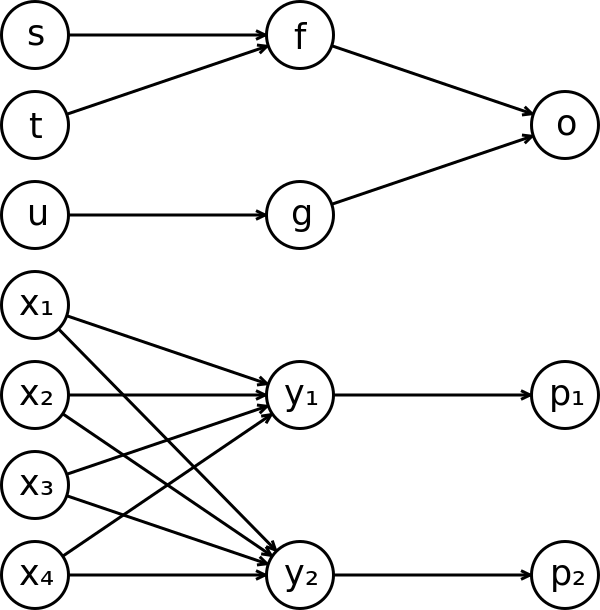
\includegraphics[scale=0.25]{sums_indep_poi_counterexample}
\caption{
    Network which yields counterexamples for POI, Strong Independence,
    PCI and Monotonicity for \sums{}
}
\label{td_fig_sums_indep_poi_counterexample}
\end{figure}
\end{proof}

The key to the counterexamples derived from
\cref{td_fig_sums_indep_poi_counterexample} in the above proof lies in the lower
connected component, which -- restricted to $\S \cup \F$ -- is a
\emph{connected} bipartite graph. That is, each source $x_i$ claims all facts
in the component, and each fact $y_j$ is claimed by all sources in the
component.  Moreover, sources elsewhere in the network claim fewer facts than
the $x_i$, and facts elsewhere are claimed by fewer sources than the $y_j$.

Since \sums{} assigns scores by a simple sum, this results in the scores for
the $x_i$ and $y_j$ dominating those of the other sources and facts. The
normalisation step then divides these scores by the (comparatively large)
maximum. As the next result shows, under certain conditions this causes scores
to decrease \emph{exponentially} and become 0 in the limit. In particular, we
can generate pathological examples such as
\cref{td_fig_sums_indep_poi_counterexample} where a whole connected component
receives scores of 0, which leads to failure of Monotonicity and the
independence axioms.

\begin{proposition}
\label{td_prop_obliteration}

Let $N$ be a network. Suppose there is $X \subseteq \S$, $Y \subseteq \F$ such
that
\begin{enumerate}
\item $\facts_N(x) = Y$ for each $x \in X$
\item $\src_N(y) = X$ for each $y \in Y$
\item $\facts_N(s) \cap Y = \emptyset$ and $|\facts_N(s)| \le \frac{|Y|}{2}$
      for each $s \in \S \setminus X$
\item $\src_N(f) \cap X = \emptyset$ and $|\src_N(f)| \le \frac{|X|}{2}$ for
      each $f \in \F \setminus Y$
\end{enumerate}
Then, with $(T^n)_{n \in \Nat}$ denoting \sums{}, for all $n > 1$ we have
    \[ T_N^n(s) \le \frac{1}{2^{n-1}} \quad (s \in \S \setminus X) \]
    \[ T_N^n(f) \le \frac{1}{2^{n-1}} \quad (f \in \F \setminus Y) \]
    \[ T_N^n(x) = 1 \quad (x \in X) \]
    \[ T_N^n(y) = 1 \quad (y \in Y) \]
In particular, if $T^*$ denotes the limit of \sums{} then $T_N^*(s) = T_N^*(f)
= 0$ for all $s \in \S \setminus X$ and $f \in \F \setminus Y$.
\end{proposition}

\begin{proof}

We proceed by induction. The result is easy to show in the base case $n = 2$
since $|\facts_N(s)| \le \frac{1}{2}|\facts_N(x)|$ for any $x \in X$ and $s
\notin X$ (and similarly for facts). Assume the result holds for some $n > 1$.
Write $T' = U^{\text{Sums}}(T^n)$, so that $T^{n+1} = \norm(T')$. If $s \notin
X$ then $\facts_N(s) \subseteq \F \setminus Y$, so
\[
    T'_N(s)
    = \sum_{f \in \facts_N(s)}{
        \underbrace{T^n_N(f)}_{\le \frac{1}{2^{n-1}}}
    }
    \le \frac{|\facts_N(s)|}{2^{n-1}}
    \le \frac{\frac{1}{2}|Y|}{2^{n - 1}}
    = \frac{|Y|}{2^{(n+1) - 1}}
\]
Similarly, if $f \notin Y$ then $\src_N(f) \subseteq \S \setminus X$, so
\[
    T'_N(f)
    = \sum_{s \in \src_N(f)}{
        \underbrace{T'_N(s)}_{\le \frac{|Y|}{2^{(n+1) - 1}}}
    }
    \le \frac{|\src_N(f)| \cdot |Y|}{2^{(n+1) - 1}}
    \le \frac{\frac{1}{2}|X| \cdot |Y|}{2^{(n+1) - 1}}
    = \frac{|X| \cdot |Y|}{2^{(n+2) - 1}}
\]

On the other hand, the fact that $T_N^n(x) = T_N^n(y) = 1$ for $x \in X$ and $y
\in Y$ gives
\[
    T'_N(x)
    = \sum_{y \in Y}{ T^n_N(y) }
    = |Y|
\]
\[
    T'_N(y) = \sum_{x \in X}{T'_N(x)} = |X| \cdot |Y|
\]
Clearly the $x \in X$ and $y \in Y$ are the sources and facts with maximal
trust and belief scores, respectively. This means that after normalisation via
$\norm$, $T_N^{n+1}(x) = T_N^{n+1}(y) = 1$ and for $s \notin X$ and $f \notin
Y$,
\[
    T_N^{n+1}(s)
    = \frac{T'_N(s)}{|Y|}
    \le \frac{1}{2^{(n+1) - 1}}
\]
\[
    T_N^{n+1}(f)
    = \frac{T'_N(f)}{|X| \cdot |Y|}
    \le \frac{1}{2^{(n+2) - 1}}
    \le \frac{1}{2^{(n+1) - 1}}
\]
This shows that the claim holds for $n+1$; by induction, the proof is complete.
\end{proof}

\subsection{Modifying \voting{} and \sums{}}
\label{td_sec_modifying_voting_and_sums}

So far we have seen that neither of the basic operators \voting{} or \sums{}
are completely satisfactory with respect to the axioms of \cref{td_sec_axioms}.
Armed with the knowledge of how and why certain axioms fail, one may wonder
whether it is possible to modify the operators accordingly so that the axioms
\emph{are} satisfied. Presently we shall show that this is partially possible
both in the case of \voting{} and \sums{}.

\subsubsection{Voting}

A core problem with \voting{} is that it fails Coherence. Indeed, all sources
are ranked equally regardless of the `votes' for facts, so in some sense it is
obvious that the source ranking does not cohere with the fact
ranking.\footnotemark{} An easy improvement is to explicitly construct the
source ranking to guarantee Source-Coherence.

% two rankings do not cohere with each other.\footnotemark{} An easy
% improvement is to ensure the rankings cohere meaningfully in at least one direction: we can
% aim for \emph{Source}-Coherence by constructing the source rankings based on
% the fact ranking of \voting{}.

\footnotetext{
    Fact-Coherence is vacuously satisfied, however: since all sources rank
    equally we can never have $\src_N(f_1)$ less trustworthy than
    $\src_N(f_2)$.
}

\begin{definition}
For a network $N$, define a binary relation $\scoh_N$ on $\S$ by $s_1
\scoh_N s_2$ iff $\facts_N(s_1)$ is less believable than
$\facts_N(s_2)$ with respect to \voting{}. The numerical operator \scvoting{}
(Source-Coherence Voting) is defined by
\[
    T_N^{SCV}(s) = |\{t \in \S : t \scoh_N s \}|,
    \quad
    T_N^{SCV}(f) = |\src_N(f)|
\]
\end{definition}

It can be seen that \scvoting{} satisfies Source-Coherence, which is a
significant improvement over regular \voting{}. Since $\scoh_N$ relies on
`global' properties on $N$, however, this comes at the expense of Source-PCI.
Satisfaction of the other axioms is inherited from \voting{}.

\begin{theorem}
\label{td_thm_scvoting_axioms}
\scvoting{} satisfies Source-Coherence, Symmetry, Unanimity, Groundedness,
Monotonicity, Fact-PCI, POI and Strong Independence. It does not
satisfy Fact-Coherence or Source-PCI.
\end{theorem}

The following properties of ${\scoh_N}$ are useful for showing
Source-Coherence.

\begin{lemma}
    $\scoh_N$ is transitive and irreflexive.
\end{lemma}

\begin{proof}

For transitivity, suppose $s \scoh_N t$ and $t \scoh_N u$. Then $\facts_N(s)$
is less believable than $\facts_N(t)$ (with respect to \voting{}) via some
bijection $\phi: \facts_N(s) \to \facts_N(t)$, and $\facts_N(t)$ is less
believable than $\facts_N(u)$ via some bijection $\psi: \facts_N(t) \to
\facts_N(u)$. It is easily seen that $\facts_N(s)$ is less believable than
$\facts_N(u)$ via the composition $\theta = \psi \circ \phi$, so $s \scoh_N u$.

For irreflexivity, suppose for contradiction that $s \scoh_N s$ for some $s \in
\S$, i.e. $F = \facts_N(s)$ is less believable than itself under some bijection
$\phi: F \to F$. Then ${f \fle_N^T \phi(f)}$ for each $f \in F$, and there is
$\hat{f}$ such that ${\hat{f} \flt_N^T \phi(\hat{f})}$. Iterating applications
of $\phi$, we get
\begin{equation}
    \label{td_eqn_iterated_phi}
    \hat{f} \flt_N^T \phi(\hat{f}) \fle_N^T \phi(\phi(\hat{f}) \fle_N^T \cdots
    \fle_N^T \phi^n(\hat{f})
\end{equation}
for each $n \ge 1$, where $\phi^n$ is the $n$-th iterate of $\phi$ and $T$
denotes \voting{}.

Since $F$ is finite, the sequence $\phi(\hat{f}), \phi(\phi(\hat{f})), \ldots$
must repeat at some point, i.e. there is $i < j$ such that
$\phi^i(\hat{f}) = \phi^j(\hat{f})$. But then injectivity of $\phi$ implies
that $\hat{f} = \phi^{j - i}(\hat{f})$. Taking $n = j - i$ in
\cref{td_eqn_iterated_phi} we get $\hat{f} \flt_N^T \hat{f}$ -- a contradiction.
\end{proof}

\begin{proof}[Proof of \cref{td_thm_scvoting_axioms} (sketch)]

Note that \scvoting{} inherits Unanimity, Groundedness, Monotonicity, Fact-PCI,
POI and Strong Independence from \voting{}, since these axioms only refer to
the rankings of facts (which is the same for \scvoting{} as for \voting{}).

We take the remaining axioms in turn. To simplify notation, write $W_N(s) = \{t
\in \S : t \scoh_N s \}$ in what follows.

\paragraph{Source-Coherence.}

Suppose $\facts_N(s_1)$ is less believable than $\facts_N(s_2)$ with respect to
$T^{SCV}$. We need to show $s_1 \slt_N^{T^{SCV}} s_2$.

Note that since the fact ranking for $T^{SCV}$ coincides with \voting{}, we
have $s_1 \scoh_N s_2$. Transitivity of ${\scoh_N}$ gives $W_N(s_1) \subseteq
W_N(s_2)$. Moreover, $s_1 \in W_N(s_2)$ but by irreflexivity, $s_1 \notin
W_N(s_1)$. Therefore $W_N(s_1) \subset W_N(s_2)$, which means $T_N^{SCV}(s_1) =
|W_N(s_1)| < |W_N(s_2)| = T_N^{SCV}(s_2)$, i.e.  $s_1 \slt_N^{T^{SCV}} s_2$ as
required.

\paragraph{Symmetry.} Since the fact ranking of $T^{SCV}$ is the same as
\voting{}, which satisfies Symmetry, we only need to show that $s_1
\sle_N^{T^{SCV}} s_2$ iff $\pi(s_1) \sle_{\pi(N)}^{T^{SCV}} \pi(s_2)$ for all
equivalent networks $N, \pi(N)$ and $s_1, s_2 \in \S$.

In can be shown, and we do so in the appendix, that the Symmetry of \voting{}
implies a symmetry property for ${\scoh_N}$ and ${\scoh_{\pi(N)}}$: we have
$s_1 \scoh_N s_2$ iff $\pi(s_1) \scoh_{\pi(N)} \pi(s_2)$. Consequently, $t \in
W_N(s_i)$ iff $\pi(t) \in W_{\pi(N)}(\pi(s_i))$; in particular, $|W_N(s_i)| =
|W_{\pi(N)}(\pi(s_i))|$. This means
\begin{align*}
    s_1 \sle_N^{T^{SCV}} s_2
    & \iff |W_N(s_1)| \le |W_N(s_2)| \\
    & \iff |W_{\pi(N)}(\pi(s_1))| \le |W_{\pi(N)}(\pi(s_2))| \\
    & \iff \pi(s_1) \sle_{\pi(N)}^{T^{SCV}} \pi(s_2)
\end{align*}
as required for Symmetry.

\paragraph{Fact-Coherence.}

\begin{figure}
    \centering
    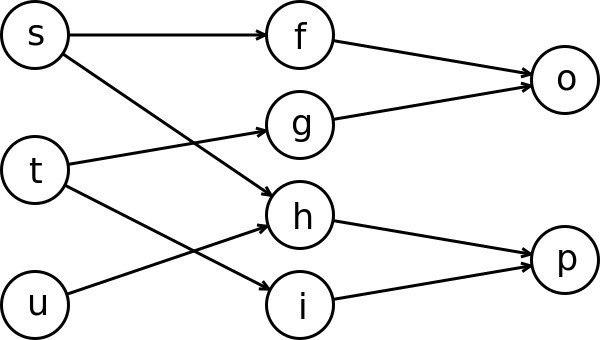
\includegraphics[scale=0.25]{scvoting_fact_coherence_counterexample}
    \caption{
        Fact-Coherence counterexample for \scvoting{}
    }
    \label{td_fig_scvoting_fact_coherence_counterexample}
\end{figure}

Consider the network shown in
\cref{td_fig_scvoting_fact_coherence_counterexample}. We have $f \feq g \feq i
\flt h$. Source-Coherence between $s$ and $t$ gives $t \slt s$. If
Fact-Coherence held we would then get $g \flt f$, but this is not the case.

\paragraph{Source-PCI.}

\begin{figure}
    \centering
    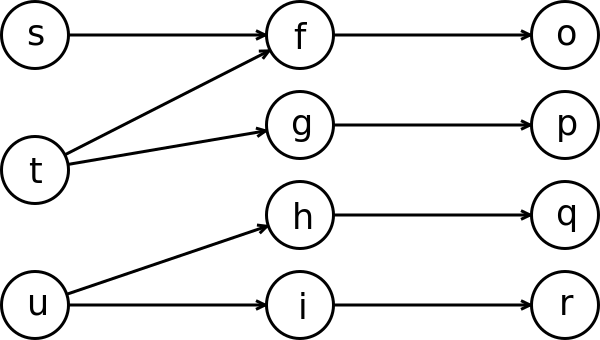
\includegraphics[scale=0.25]{scvoting_independence_counterexample}
    \caption{
        Source-PCI counterexample for \scvoting{}
    }
    \label{td_fig_scvoting_independence_counterexample}
\end{figure}

Let $N_1$ denote the top connected component of the network shown in
\cref{td_fig_scvoting_independence_counterexample}, and let $N_2$ denote the
network as a whole. The fact ranking is the same in both networks: $g \feq h
\feq i \flt f$.  In $N_1$ sources $s$ and $t$ claim a different number of
facts, so neither $s \scoh_{N_1} t$ nor $t \scoh_{N_1} s$. Consequently
$W_{N_1}(s) = W_{N_1}(t) = \emptyset$ and $s \seq_{N_1}^{T^{SCV}} t$.

In $N_2$ sources $t$ and $u$ can be compared for Source-Coherence, and we see
that $u \scoh_{N_2} t$ since $i \fle_{N_2}^{T^{SCV}} g$ and $h
\flt_{N_2}^{T^{SCV}} f$. Hence $W_{N_2}(t) = \{u\}$ and $W_{N_2}(s) =
\emptyset$, which means $s \slt_{N_2}^{T^{SCV}} t$. This contradicts
Source-PCI, which requires the ranking of $s$ and $t$ to be the same in both
networks.  \end{proof}

Note that the idea behind \scvoting{} can be generalised
beyond \voting{}: it is possible to define $\scoh_N$ in terms of \emph{any}
operator $T$, and to construct a new operator $T'$ whose source ranking is
given according to $\scoh_N$ as above, and whose fact ranking coincides with
that of $T$. This ensures $T'$ satisfies Source-Coherence whilst keeping the
existing fact ranking from $T$.

Moreover we can go in the other direction and ensure \emph{Fact}-Coherence
whilst retaining the source ranking of $T$ by defining a relation $\fcoh_N$ on
$\F$ in a analogous manner to $\scoh_N$, and proceeding similarly.

\subsubsection{Sums}

Our main concern with \sums{} is the failure of PCI and Monotonicity.  We have
seen that this is in some sense caused by the normalisation step: in
\cref{td_fig_sums_indep_poi_counterexample} the scores of $f, g$ etc go to 0 in
the limit after dividing the `global' maximum score across the network, which
happens to come from a different connected component.

A natural fix for PCI is to therefore divide by the maximum score
\emph{within each component}. In this case the score for a source $s$ depends
only on the structure of the connected component in which it lies, which is
exactly what is required for PCI.

However, this approach does not negate the undesirable effects of
\cref{td_prop_obliteration}. Indeed, suppose the network in
\cref{td_fig_sums_indep_poi_counterexample} was modified so that fact $y_1$ is
associated with object $o$ instead of $p_1$. Clearly \cref{td_prop_obliteration}
still applies after this change, and all sources and facts shown now belong to
the same connected component. Therefore the `per-component \sums{}' operator
gives the same result as \sums{} itself, and in particular our Monotonicity
counterexample still applies. Perhaps even worse, one can show that Coherence
fails for this operator. We consider the loss of Coherence too high a price to
pay for PCI.

Instead, let us take a step back and consider if normalisation is truly
necessary. On the one hand, without normalisation the trust and belief scores
are unbounded and therefore do not converge. On the other, we are not
interested in the numeric scores for their own sake, but rather for the
\emph{rankings} that they induce. It may be possible that whilst the scores
diverge without normalisation, the induced rankings \emph{do} converge to a
fixed one, which we may take as the `ordinal limit'. This is in fact the case.
We call this new operator \usums{}.

\begin{definition}

\usums{} is the recursive operator $\rec(T^{\text{prior}}, U^{\text{Sums}})$
where $T_N^{\text{prior}}(s) = 1$, $T_N^{\text{prior}}(f) = |\src_N(f)|$ and
$U^{\text{Sums}}$ is defined as in \cref{td_sec_sums_example}.\footnotemark{}

\end{definition}

\footnotetext{
    Note that to simplify proof of ordinal convergence we use a different prior
    operator to \sums{}, but this does not effect the operator in any
    significant way.
}



\begin{theorem}
\label{td_thm_usums_ordinal_convergence}
\usums{} is ordinally convergent in the following sense: there is an ordinal
operator $T^*$ such that for each network $N$ there exists $J_N \in \Nat$ such
that $T_N^n(s_1) \le T_N^n(s_2)$ iff $s_1 \sle_N^{T^*} s_2$ for all $n \ge J_N$
and $s_1, s_2 \in \S$ (and similarly for facts).

That is, the rankings induced by $T^n$ remain constant after $J_N$ iterations,
and are identical to those of $T^*$.
\end{theorem}

\begin{proof}
    The proof will use some results from linear algebra, so we will work with a
    matrix and vector representation of \usums{}. Fix an enumeration $\S =
    \{s_1,\ldots,s_k\}$ of $\S$ and $\F = \{f_1,\ldots,f_l\}$ of $\F$. Write
    $M$ for the $k \times l$ matrix given by
    \[
        [M]_{ij} = \begin{cases}
            1 & \text{ if } s_i \in \src_N(f_j) \\
            0 & \text{ otherwise }
        \end{cases}
        \quad
        (1 \le i \le k, 1 \le j \le l)
    \]
    We also write $v_n$ and $w_n$ for the vectors of trust and belief scores of
    \usums{} at iteration $n$; that is
    \[
        v_n = [T_N^n(s_1), \ldots, T_N^n(s_k)]^\top \in \R^k
    \]
    \[
        w_n = [T_N^n(f_1), \ldots, T_N^n(f_l)]^\top \in \R^l
    \]
    where $(T^n)_{n \in \Nat}$ denotes \usums{}.

    Multiplication by $M$ encodes the update step of \usums{}: it is easily
    shown that $v_{n+1} = Mw_n$ and $w_{n+1} = M^{\top}v_{n+1}$.  Writing $A =
    MM^\top \in \R^{k \times k}$, we have $v_{n+1} = Av_n$, and therefore
    $v_{n+1} = A^n v_1$.

    To show that the rankings of \usums{} remain constant after finitely many
    iterations, we will show that for each $s_p, s_q \in \S$ there is $J_{pq}
    \in \Nat$ such that $\sign([v_n]_p - [v_n]_q)$ is constant for all $n \ge
    J_{pq}$. Since $[v_n]_p$ and $[v_n]_q$ are the trust scores of $s_p$ and
    $s_q$ respectively in the $n$-th iteration, this will show that the ranking
    of $s_p$ and $s_q$ remains the same after $J_{pq}$ iterations. Since there
    are only finitely many pairs of sources, we may then take $J_N$ as the
    maximum value of $J_{pq}$ over all pairs $(p, q)$, and the entire source
    ranking ${\sle_N^{T^n}}$ of \usums{} remains constant for $n \ge J_N$. An
    almost identical argument can be carried out for the fact ranking, and
    these together will prove the result.

    So, fix $s_p, s_q \in \S$. Write $\delta_n = [v_n]_p - [v_n]_q$. First note
    that $A = MM^\top$ is symmetric, so the \emph{spectral theorem} gives the
    existence of $k$ orthogonal eigenvectors $x_1, \ldots, x_k$ for
    $A$~\cite[Theorem 7.29]{axler2014}. Let $\lambda_1, \ldots, \lambda_k$ be
    the corresponding eigenvalues. Form a $(k \times k)$-matrix $P$ whose
    $i$-th column is $x_i$, and let $D =
    \text{diag}(\lambda_1,\ldots,\lambda_k)$. Then $A$ can be diagonalised as
    $A = PDP^{-1}$. It follows that for any $n \in \Nat$, $A^n = PD^nP^{-1}$.

    Now, since $x_1,\ldots,x_k$ are orthogonal, $P$ is an orthogonal matrix, i.e.
    $P^\top = P^{-1}$. Hence $A^n = PD^nP^\top$. Note that
    \[
        PD^n
        = \begin{bmatrix}
            x_1 \mid \ldots \mid x_k
        \end{bmatrix}
        \begin{bmatrix}
            \lambda_1^n &        &             \\
                        & \ddots &             \\
                        &        & \lambda_k^n \\
        \end{bmatrix}
        = \begin{bmatrix}
            \lambda_1^n x_1 \mid \ldots \mid \lambda_k^n x_k
        \end{bmatrix}
    \]
    and
    \[
        P^{\top}v_1
        = \begin{bmatrix}
            x_1 \\ - \\ \vdots \\ - \\ x_k
        \end{bmatrix} v_1
        = \begin{bmatrix}
            x_1 \cdot v_1 \\ \vdots \\ x_k \cdot v_1
        \end{bmatrix}
    \]
    which means
    \[
        v_{n+1}
        = A^nv_1
        = PD^nP^{\top}v_1
        = \begin{bmatrix}
            \lambda_1^n x_1 \mid \ldots \mid \lambda_k^n x_k
        \end{bmatrix}
        \begin{bmatrix}
            x_1 \cdot v_1 \\ \vdots \\ x_k \cdot v_1
        \end{bmatrix}
        = \sum_{i=1}^{k}{(x_i \cdot v_1) \lambda_i^n x_i}
    \]
    We obtain an explicit formula for $\delta_{n+1}$:
    \begin{equation}
        \label{td_eqn_delta_formula}
        \delta_{n+1}
        = [v_n]_p - [v_n]_q
        = \sum_{i=1}^{k}{
            (x_i \cdot v_1) \lambda_i^n \left( [x_i]_p - [x_i]_q \right)
        }
        = \sum_{i=1}^{k}{r_i \lambda_i^n}
    \end{equation}
    where $r_i = (x_i \cdot v_1)\left( [x_i]_p - [x_i]_q \right)$. Note that
    $r_i$ does not depend on $n$.

    Now, it is easy to see that $A = MM^\top$ is \emph{positive semi-definite},
    which means its eigenvalues $\lambda_1,\ldots,\lambda_k$ are all
    non-negative. We re-index the sum in \cref{td_eqn_delta_formula} by grouping
    together the $\lambda_i$ which are equal, to get
    \[
        \delta_{n+1} = \sum_{t=1}^{K}{R_t \mu_t^n}
    \]
    where $K \le k$, each $R_t$ is a sum of the $r_i$ (whose corresponding
    $\lambda_i$ are equal), and the $\mu_t$ are distinct and non-negative.
    Assume without loss of generality that $\mu_1 > \mu_2 > \cdots > \mu_K \ge
    0$. If $R_t = 0$ for all $t$, then clearly $\sign(\delta_{n+1}) = \sign(0)
    = 0$ which is constant, so we are done. Otherwise, let $T$ be the minimal
    $t$ such that $R_t \ne 0$. We may also assume $\mu_T > 0$ (otherwise we
    necessarily have $\mu_T = 0$, $T=K$ and $\sign(\delta_{n+1}) = \sign(R_T
    \cdot 0^n)$ which is again constant 0). Observe that
    \[
        \delta_{n+1}
        = R_T \mu_T^n + \sum_{t=T + 1}^{K}{R_t \mu_t^n} \\
        = \mu_T^n \left[
            R_T + \sum_{t=T + 1}^{K}{
                R_t \left(\frac{\mu_t}{\mu_T}\right)^n
            }
        \right]
    \]
    By our assumption on the ordering of the $\mu_t$, we have $\mu_t < \mu_T$
    in the sum. Consequently $|\mu_t / \mu_T| < 1$, and $(\mu_t / \mu_T)^n \to
    0$ as $n \to \infty$. This means
    \[
        \limn{\left[
            R_T + \sum_{t=T + 1}^{K}{
                R_t \underbrace{\left(\frac{\mu_t}{\mu_T}\right)^n}_{\to 0}
            }
        \right]}
        = R_T
        \ne 0
    \]
    Since this limit is non-zero, there is $J_{pq} \in \Nat$ such that the sign
    of term in square brackets is
    equal to $S = \sign R_T \in \{1, -1\}$ for all $n \ge J_{pq}$. Finally,
    for such $n$ we have
    \[
        \sign \delta_{n+1}
        = \sign \left(
            \underbrace{\mu_T^n}_{> 0}
            \left[
                R_T + \sum_{t=T + 1}^{K}{
                    R_t \left(\frac{\mu_t}{\mu_T}\right)^n
                }
            \right]
        \right)
        = \sign \left(
            R_T + \sum_{t=T + 1}^{K}{
                R_t \left(\frac{\mu_t}{\mu_T}\right)^n
            }
        \right)
        = S
    \]
    i.e. $\sign \delta_n$ is constant for $n \ge J_{pq} + 1$. This completes
    the proof.\footnote{
        The argument which shows that the difference between fact belief scores
        is also eventually constant in sign is almost identical. Write $B =
        M^{\top}M$, and observe that $w_{n+1} = B^nw_1$. Since $B$ is also
        symmetric and positive semi-definite, the proof goes through as above.
    }
\end{proof}

In light of \cref{td_thm_usums_ordinal_convergence}, we may consider \usums{}
itself as an ordinal operator $T^*$, where $s \sle_N^{T^*} t$ iff $s
\sle_N^{T^{J_n}} t$ for each network $N$ (and similarly for the fact ranking).
Moreover, with the normalisation problems aside, \usums{} provides an example
of a principled operator satisfying our two key axioms -- Coherence and PCI. In
particular, we escape the undesirable behaviour of \sums{} in
\cref{td_fig_sums_indep_poi_counterexample}; whereas \sums{} trivialises the
ranking of sources and facts in the upper connected component, \usums{} allows
meaningful ranking (e.g. we have $g \flt f$). In particular, the counterexample
for Monotonicity for \sums{} is no longer a counterexample for \usums{}. We
conjecture that \usums{} also satisfies Monotonicity, but this remains to be
proven. For example, we have experimentally verified that \usums{} satisfies
all the specific instances of Monotonicity with the starting network $N$ as in
\cref{td_fig_intro_example}.

\begin{theorem}
\label{td_thm_usums_axioms}
\usums{} satisfies Coherence, Symmetry, Unanimity, Groundedness and
PCI. \usums{} does not satisfy POI and Strong Independence.
\end{theorem}

\begin{proof}[Proof (sketch)]
% \begin{proof}[Proof (sketch)]

The proof that \usums{} satisfies Symmetry, PCI, Unanimity and Groundedness is
routine, and we leave the details to the appendix. In what follows, let
$(T^n)_{n \in \Nat}$ denote \usums{}, $T^*$ denote the ordinal limit of
\usums{}, and for a network $N$ let $J_N$ be as in
\cref{td_thm_usums_ordinal_convergence}. Then the rankings in $N$ induced by $T^n$
for $n \ge J_N$ are the same as $T^*$.

\paragraph{Coherence.}
First we show Source-Coherence. Let $N$ be a network and suppose
$\facts_N(s_1)$ is less believable than $\facts_N(s_2)$ with respect to $N$ and
$T^*$. Let $\phi$ and $\hat{f}$ be as in the definition of less believable.

Let $n \ge J_N$. Then $f \fle_N^{T^*} \phi(f)$ and $\hat{f} \flt_N^{T^*}
\phi(\hat{f})$ for each $f \in \facts_N(s_1)$ means $T_N^n(f) \le
T_N^n(\phi(f))$ and $T_N^n(\hat{f}) < T_N^n(\phi(\hat{f}))$. Hence
\begin{align*}
    T_N^{n+1}(s)
    &= \sum_{f \in \facts_N(s_1)}{T_N^n(f)} \\
    &= T_N^n(\hat{f}) + \sum_{f \in \facts_N(s_1) \setminus \{\hat{f}\}}{T_N^n(f)} \\
    &< T_N^n(\phi(\hat{f})) + \sum_{f \in \facts_N(s_1) \setminus \{\hat{f}\}}{T_N^n(\phi(f))} \\
    &= \sum_{f \in \facts_N(s_1)}{T_N^n(\phi(f))} \\
    &= \sum_{g \in \facts_N(s_2)}{T_N^n(g)} \\
    &= T_N^{n+1}(s_2)
\end{align*}
i.e. $T_N^{n+1}(s_1) < T_N^{n+1}(s_2)$. But $T_N^{n+1}$ gives the same ranking
as $T_N^n$ and therefore the same ranking as $T^*$, so we get $s_1 \slt_N^{T^*}
s_2$ as required.

For Fact-Coherence, suppose $\src_N(f_1)$ is less trustworthy than
$\src_N(f_2)$ with respect to $N$ and $T^*$. Again, let $n \ge J_N$ and $\phi$,
$\hat{s}$ be as in the definition of less trustworthy. Recall that belief
scores for facts in $T_N^n$ are obtained from trust scores in $T_N^n$; applying
the same argument as above we get $T_N^n(f_1) < T_N^n(f_2)$ and consequently
$f_1 \fle_N^{T^*} f_2$ as required. Hence $T^*$ satisfies Coherence.

\paragraph{POI and Strong Independence.}

\begin{figure}[ht]
\centering
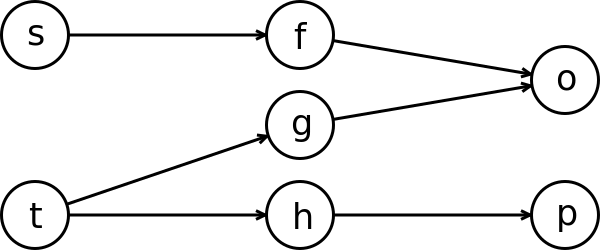
\includegraphics[scale=0.25]{usums_poi_counterexample}
\caption{
    Counterexample for POI and Strong Independence for \usums{}
}
\label{td_fig_usums_poi_counterexample}
\end{figure}

To show POI and Strong Independence are not satisfied, consider the network $N$
shown in \cref{td_fig_usums_poi_counterexample}. It can be seen (e.g. by
induction) that
\[
    T_N^n(f) = 1,
    \quad
    T_N^n(g) = 2^{n-1}
\]
for all $n \in \Nat$. Consequently $f \flt_N^{T^*} g$.\footnotemark

\footnotetext{
    Note that $g$ ranks higher than $f$ in this network simply because $t$
    makes more claims than $s$, and each fact is claimed only by a single
    source. This questionable property of \usums{} is inherited from \sums{}.
}

Now let $N'$ be the network in which the claim $(t, h)$ is removed. Since
$\src_N(f) = \src_{N'}(f) = \{s\}$ and $\src_N(g) = \src_{N'}(g) = \{t\}$, both
POI and Strong Independence imply $f \fle_N^{T^*} g$ iff $f \fle_{N'}^{T^*} g$.
Therefore assuming either of POI or Strong Independence we get $f
\flt_{N'}^{T^*} g$. However is is also clear that
\[
    T_{N'}^n(f) = T_{N'}^n(g) = 1
\]
for all $n \in \Nat$, so $f \feq_{N'}^{T^*} g$. This is a contradiction, so
neither POI nor Strong Independence are satisfied.
\end{proof}

To summarise this section, \cref{td_table_axioms} shows which axioms are
satisfied by each of the operators.

\begin{table}
\newcommand{\yes}{\checkmark}
\newcommand{\no}{\sffamily{X}}
\newcommand{\notsure}{?}
\centering
    \caption{Satisfaction of the axioms for the various operators. Recall that
    POI and Strong Independence are undesirable properties.}
    \begin{tabular}{c c c c c}
        \toprule
                         & Voting & SC-Voting  & Sums & U-Sums   \\
        \midrule
        Source-Coherence & \no    & \yes       & \yes & \yes     \\
        Fact-Coherence   & \yes   & \no        & \yes & \yes     \\
        Symmetry         & \yes   & \yes       & \yes & \yes     \\
        Unanimity        & \yes   & \yes       & \yes & \yes     \\
        Ground.          & \yes   & \yes       & \yes & \yes     \\
        Mon.             & \yes   & \yes       & \no  & \notsure \\
        Source-PCI       & \yes   & \no        & \no  & \yes     \\
        Fact-PCI         & \yes   & \yes       & \no  & \yes     \\
        \hline
        POI              & \yes   & \yes       & \no  & \no      \\
        Str. Indep.      & \yes   & \yes       & \no  & \no      \\
        \bottomrule
    \end{tabular}
\label{td_table_axioms}
\end{table}

\section{Variable domain truth discovery}
\label{td_sec_variable_domain}

So far, we have considered an arbitrary but fixed (finite) domain of sources,
facts and objects $(\S, \F, \O)$. Our operators and axioms were defined with
respect to this domain. However, the operators do not \emph{depend} on the
domain: they can be defined for \emph{any} choice of $\S$, $\F$ and $\O$. In
this section we generalise the framework so that these sets are no longer
fixed. This allows new situations to be modelled, such as new sources entering
the network. Adapting the definition of a TD operator to this case, we can then
see how the ranking of facts changes as new sources are added. Such variable
domain operators are then analogues of \emph{variable electorate voting rules}
in social theory.

Formally, let $\uS$, $\uF$ and $\uO$ be countably infinite sets of sources,
facts and objects respectively. A \emph{domain} is a triple $\D = (\S, \F,
\O)$, where $\S \subseteq \uS$, $\F \subseteq \uF$ and $\O \subseteq \uO$ are
finite, non-empty sets. We think of $\uS$, $\uF$ and $\uO$ as being the
`universe' of possible sources, facts and objects, and a domain as the (finite)
sets of entities under consideration in a particular TD problem. Given a domain
$\D = (\S, \F, \O)$, we define $\D$-networks and $\D$-operators as in
\cref{def_td_network,td_def_truth_discovery_operator}.

\begin{definition}
    A \emph{variable domain operator} $T$ is a mapping which maps each domain
    $\D$ to a $\D$-operator $T_\D$.
\end{definition}

Note that for a domain $\D = (\S, \F, \O)$ and a $\D$-network $N$,
$\sle_N^{T_\D}$ and $\fle_N^{T_\D}$ are rankings only over the set of sources
$\S$ and $\F$ in the domain $\D$, \emph{not} all of $\uS$ and $\uF$. If $\D$ is
clear from context, we write $\sle_N^T$ and $\fle_N^T$ without explicit
reference to the domain.

Since all the axioms so far were stated with respect to a fixed but arbitrary
domain, they can be easily lifted to the variable domain case. For instance, we
say a variable domain operator $T$ satisfies Coherence if $T_\D$ satisfies the
instance of Coherence for domain $\D$, for all $\D$, and similar for the other
axioms.

But we can now go further, and introduce axioms which make use of
\emph{several} domains. First, we generalise Symmetry to act across domains.
Say networks $N, N'$ in domains $\D, \D'$ respectively are \emph{equivalent} if
there is a graph isomorphism $\pi$ between them such that $\pi(s) \in \S'$,
$\pi(f) \in \F'$ and $\pi(o) \in \O'$ for all $s \in \S$, $f \in \F$ and $o \in
\O$.

\begin{axiom}[Isomorphism]
    Let $N$ and $N' = \pi(N)$ be equivalent networks. Then for all $s_1, s_2
    \in \S$, $f_1, f_2 \in \F$, we have $s_1 \sle_N^T s_2$ iff $\pi(s_1)
    \sle_{N'}^T \pi(s_2)$ and $f_1 \fle_N^T f_2$ iff $\pi(f_1) \fle_{N'}^T
    \pi(f_2)$.
\end{axiom}

Like Symmetry, Isomorphism simply says that operators only care about the
\emph{structure} of the network, not the particular `names' chosen for sources,
facts and objects. Symmetry is obtained as the special case where $N$ and $N'$
are equivalent when seen as networks in a common domain $\D$. All the operators
of \cref{td_sec_specific_operators,td_sec_modifying_voting_and_sums} satisfy
Isomorphism.

Next we introduce a new monotonicity property. In what follows, for a network
$N = (V, E)$ in domain $(\S, \F, \O)$, $f \in \F$ and $\S' \subseteq \uS$
finite and disjoint from $\S$, write $N + (\S', f)$ for the network in domain
$(\S \cup \S', \F, \O)$ with edge set $E \cup \{(s, f) \mid s \in \S'\}$, i.e.
the extension of $N$ where a collection of `fresh' sources $\S'$ each claim
$f$. For example, \cref{td_fig_eventual_mon_example} shows $N + (\S', h)$ for the
network $N$ from \cref{td_fig_intro_example} and new sources $\S' = \{x_1, \ldots,
x_4\}$.

\begin{figure}[b]
\centering
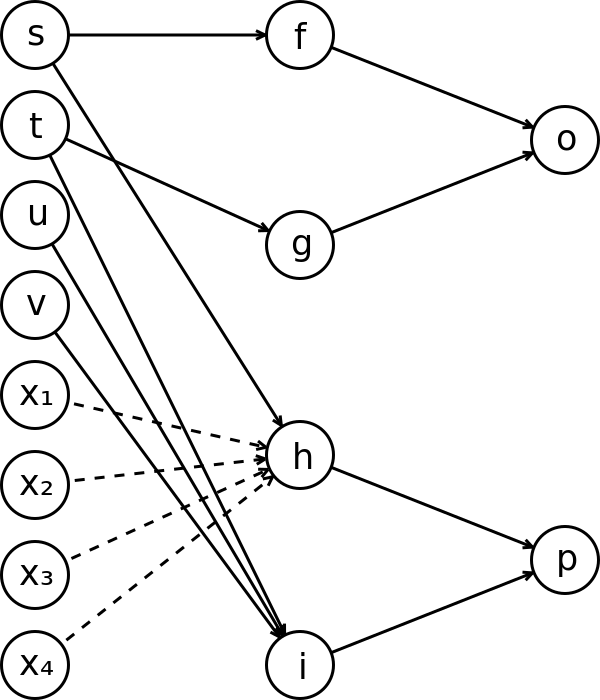
\includegraphics[scale=0.25]{eventual_mon_example}
\caption{
    $N + (\S', h)$, where $N$ is the network from \cref{td_fig_intro_example} and
    $\S' = \{x_1, \ldots, x_4\}$.
}
\label{td_fig_eventual_mon_example}
\end{figure}

\begin{axiom}[Eventual Monotonicity]
    Let $\D = (\S, \F, \O)$ be a domain and $N$ a $\D$-network. Then for all
    $f, g \in \F$, $f \ne g$, there is a finite, non-empty set $\S' \subseteq
    \uS$ with $\S \cap \S' = \emptyset$ and $g \flt_{N + (\S', f)}^T f$.
\end{axiom}

This axiom says that, given any pair of distinct facts $f, g$, it is possible
to add enough new claims for $f$ to make $f$ strictly more believable than $g$.
Intuitively, this is less demanding that Monotonicity, which requires that $f$
can become strictly more believable than $g$ with the addition of just
\emph{one} additional claim. Note that Eventual Monotonicity is not possible to
state in the fixed domain case (e.g. consider $N$ already containing claims
from all the available sources in $\S$).

When paired with Isomorphism, Eventual Monotonicity takes on a form similar to
postulates for \emph{Improvement} and \emph{Majority} operators in belief
merging~\cite{koniecznyP08_improvement,konieczny2002merging}: there is a
threshold $n \in \Nat$ such that $f$ becomes strictly more believable than $g$
after $n$ new claims are added for $f$. That is, the identities of the new
sources $\S'$ are irrelevant; it is just the \emph{size} of $\S'$ that matters.
We require a preliminary lemma.

\begin{lemma}
    \label{td_lemma_isomorphism_var_op}
    Suppose a variable domain operator $T$ satisfies Isomorphism. Let $\D = (\S,
    \F, \O)$ be a domain, $N$ a network in $\D$ and $f \in \F$. Then for all
    non-empty, finite sets $\S'_1, \S'_2 \subseteq \uS$ disjoint from $\S$ with
    $|\S'_1| = |\S'_2|$,
    \[
        {\fle_{N + (\S'_1, f)}^T}
        =
        {\fle_{N + (\S'_2, f)}^T}
    \]
\end{lemma}

\begin{proof}
    Write $\D_1 = (\S \cup \S'_1, \F, \O)$ and $\D_2 = (\S \cup \S'_2, \F,
    \O)$. Then $N + (\S'_i, f)$ is a network in domain $\D_i$ (for $i \in \{1,
    2\}$). Since $|\S'_1| = |\S'_2|$ by assumption, there is a bijection $\phi:
    \S'_1 \to \S'_2$. Define a mapping $\pi$ from $\D_1$ to $\D_2$ by
    \[
        \pi(s) = \begin{cases}
            s,& s \in \S \\
            \phi(s),& s \in \S'_1
        \end{cases}
        \quad (s \in \S \cup \S'_1)
    \]
    and $\pi(g) = g$, $\pi(o) = o$ for $g \in \F$ and $o \in \O$. Then it is
    easily verified that $\pi$ is an isomorphism from $N + (\S'_1, f)$ to $N +
    (\S'_2, f)$. For $g_1, g_2 \in \F$, we have $g_1 \fle_{N + (\S'_1, f)}^T
    g_2$ iff $\pi(g_1) \fle_{N + (\S'_2, f)}^T \pi(g_2)$ by Isomorphism. Since
    $\pi(g_1) = g_1$ and $\pi(g_2) = g_2$, this shows ${\fle_{N + (\S'_1,
    f)}^T} = {{\fle_{N + (\S'_2, f)}^T}}$.
\end{proof}

Note that since $\uS$ is infinite and domains are finite, for any $n \in \Nat$
and any domain $\D = (\S, \F, \O)$ there is always some $\S' \subseteq \uS$,
disjoint from $\S$, with $|\S'| = n$. For operators $T$ satisfying Isomorphism,
write $\fle_{N + (n \times f)}^T$ for $\fle_{N + (\S', f)}^T$;
\cref{td_lemma_isomorphism_var_op} guarantees this is well-defined (i.e. does not
depend on the particular choice of $\S'$). That is, $\fle_{N + (n \times f)}^T$
is the fact ranking resulting from adding $n$ new claims for $f$ from fresh
sources. We obtain an equivalent characterisation of Eventual Monotonicity,
whose proof is almost immediate given \cref{td_lemma_isomorphism_var_op}.

\begin{proposition}
    \label{td_prop_eventual_mon_iff_improvement}
    Suppose $T$ satisfies Isomorphism. Then $T$ satisfies Eventual Monotonicity
    if and only if for all domains $\D = (\S, \F, \O)$, all networks $N$ in
    $\D$ and distinct $f, g \in \F$, there is $n \in \Nat$ such that $g \flt_{N
    + (n \times f)}^T f$.
\end{proposition}

\begin{proof}
    `if': To show Eventual Monotonicity, take any $\S' \subseteq \uS \setminus
    \S$ of size $n$.

    `Only if': Given that Eventual Monotonicity holds, simply take $n = |\S'|$.
\end{proof}

We can now show that all operators studied so far -- when lifted to the
variable domain case -- satisfy Eventual Monotonicity.

\begin{theorem}
    \label{td_thm_operators_satisfy_eventual_mon}
    \voting{}, \sums{}, \scvoting{} and \usums{} satisfy Eventual Monotonicity.
\end{theorem}

\begin{proof}[Proof (sketch)]
    Let $\D = (\S, \F, \O)$ be a domain, $N$ a network in $\D$ and $f, g \in
    \F$. Given that Isomorphism holds for each operator, we sketch the proof
    via \cref{td_prop_eventual_mon_iff_improvement}.

    For \voting{} and \scvoting{}, we may simply take $n = 1 + |\src_N(g)|$.
    For \sums{} and \usums{}, take $n = 2 |\S| \cdot |\F|$. Write $N' = N +
    (\S', f)$ for some $\S' \subseteq \uS \setminus \S$ with $|\S'| = n$

    If $(T^k)_{k \in \Nat}$ denotes \sums{}, one can show by induction that
    $T^k_{N'}(f) = 1$ and $T^{k}_{N'}(h) \le \frac{1}{2}$ for any $h \ne f$ and
    $k > 1$, and thus $g \flt_{N'}^{T^\sums{}} f$.

    Similarly, letting $(T^k)_{k \in \Nat}$ denote \usums{}, one can show by
    induction that $T^{k}_{N'}(f) > T^{k}_{N'}(h)$ for $h \ne f$, and thus $g
    \flt_{N'}^{T^\usums{}} g$.
\end{proof}

To conclude this section, we show that the impossibility result of
\cref{td_thm_impossibility} holds in the variable domain case if one replaces
Monotonicity with Eventual Monotonicity and Symmetry with Isomorphism.

\begin{theorem}
\label{td_thm_var_dom_impossibility}
    There is no variable domain operator satisfying Coherence, Isomorphism,
    Eventual Monotonicity and POI.
\end{theorem}

\begin{proof}
    For contradiction, suppose $T$ is an operator satisfying the stated axioms.
    Let $N$ be the network from \cref{td_fig_intro_example}, viewed as a network
    in domain $(\{s, t, u, v\}, \{f, g, h, i\}, \{o, p\})$. Applying Eventual
    Monotonicity with $i$ and $h$, we have that there is $N'$ with $i
    \flt_{N'}^T h$, where $N' = N + (\S', h)$ for some $\S' \subseteq \uS
    \setminus \{s, t, u, v\}$. Since $N'$ only adds claims for $p$-facts, POI
    applied to object $o$ and Isomorphism give $f \feq_{N'}^T g$ (e.g. consider
    $\pi$ which simply swaps $s$ with $t$ and $f$ with $g$). From
    Source-Coherence we get $t \slt_{N'}^T s$. But $\src_{N'}(f) = \{s\}$ and
    $\src_{N'}(g) = \{t\}$, so Fact-Coherence gives $g \flt_{N'}^T f$:
    contradiction!
\end{proof}

\section{Discussion}
\label{td_sec_discussion}

In this section we discuss the axioms and their limitations.
%
First, the version of Monotonicity we consider is a strict one: a new claim for
$f$ gives $f$ a \emph{strictly} positive boost in the fact believability
ranking. This is also the case for Eventual Monotonicity in the variable domain
case, where we require that some number of new claims make $f$ strictly more
believable than any other fact $g$. As noted in \cref{td_sec_fact_ranking_axioms},
this assumes there is no \emph{collusion} between sources. Indeed, suppose
sources $s_1$, $s_2$ are in collusion. For example, $s_2$ may agree to
unconditionally back up all claims made by $s_1$. In this case a claim of $f$
from $s_1$ alone should carry just as much weight as the claim from both $s_1$
and $s_2$. However, Monotonicity requires that $f$ becomes strictly more
believable when moving to the latter case.

A natural solution is to simply relax the strictness requirement. We obtain the
following weak version of Monotonicity.

\begin{axiom}[Weak Monotonicity]
Let $N, s, f, N'$ be as in the statement of Monotonicity. Then for all $g \ne
f$, $g \fle_N^T$ implies $g \fle_{N'}^T f$.
\end{axiom}

Weak Monotonicity only says says that extra support for a fact $f$ does not
make $f$ \emph{less} believable. Clearly Monotonicity implies Weak
Monotonicity, but not vice versa. In the collusion example, an operator may
select to leave the fact ranking unchanged when a new report of $f$ from $s_2$
arrives; this is inconsistent with Monotonicity but consistent with Weak
Monotonicity. The weak analogue of Eventual Monotonicity can be defined in the
same way.

In the same spirit, one could consider versions of Coherence only using weak
comparisons. Say $\facts_N(s_1)$ is \emph{weakly less believable} than
$\facts_N(s_2)$ iff the condition in \cref{td_def_coherence_less_believable}
holds, but without the requirement that some $\hat{f} \in \facts_N(s_1)$ is
strictly less believable than its counterpart $\phi(\hat{f})$ in
$\facts_N(s_2)$, and define $\src_N(f_1)$ weakly less trustworthy than
$\src_N(f_2)$ in a similar way. The weak analogue of Coherence is as follows.

\begin{axiom}[Weak Coherence]

For any network $N$, $\facts_N(s_1)$ weakly less believable than
$\facts_N(s_2)$ implies $s_1 \sle_N^T s_2$, and $\src_N(f_1)$ weakly less
trustworthy than $\src_N(f_2)$ implies $f_1 \fle_N^T f_2$.

\end{axiom}

Note that Coherence does \emph{not} imply Weak Coherence. This is because Weak
Coherence relaxes both the consequent \emph{and the antecedent} in the
implications in the statement of the axiom. Whereas Coherence imposes no
constraint when $\facts_N(s_1)$ is only weakly less believable than
$\facts_N(s_2)$, Weak Coherence requires $s_1 \sle_N^T s_2$. Consequently, the
`weakness' of Weak Coherence refers to its use of weak comparisons between
sources and facts, not its logical strength in relation to Coherence.

A natural question now arises. Does the impossibility result of
\cref{td_thm_impossibility} still hold with these new axioms? We have an answer in
the negative: the `flat' operator, which sets all sources and facts equally
ranked in all networks, satisfies all the axioms of the would-be impossibility.

\begin{proposition}
    Define an operator $T$ by $s_1 \seq_N^T s_2$ and $f \feq_N^T f_2$ for all
    networks $N$, sources $s_1, s_2$ and facts $f_1, f_2$. Then $T$ satisfies
    Coherence, Weak Coherence, Symmetry, Weak Monotonicity and POI.
\end{proposition}

\begin{proof}
    Coherence holds vacuously since we can never have $\facts_N(s_1)$ less
    believable than $\facts_N(s_2)$ or $\src_N(f_1)$ less believable than
    $\src_N(f_2)$. Since \emph{any} weak ranking holds for $T$, the other
    axioms are straightforward to see.
\end{proof}

This shows that (strict) Monotonicity is required for the impossibility result,
since the result is no longer true when relaxing to Weak Monotonicity.

We now consider the new axioms in relation to the operators. First, Weak
Coherence.

\begin{proposition}
    \label{td_prop_weak_coherence_satisfaction}
    \voting{}, \sums{} and \usums{} satisfy Weak Coherence
\end{proposition}

\begin{proof}[Proof (sketch)]\leavevmode

    \paragraph{\voting{}.} Since $s_1 \sle_N^{T^\voting{}} s_2$ always holds,
    Weak Source-Coherence clearly holds. For Weak Fact-Coherence, suppose
    $\src_N(f_1)$ is weakly less trustworthy than $\src_N(f_2)$. Then there is
    a bijection $\phi: \src_N(f_1) \to \src_N(f_2)$, so $|\src_N(f_1)| =
    |\src_N(f_2)|$. By definition of \voting{}, $f_1 \feq_N^{T^\voting{}} f_2$.
    In particular, $f_1 \flt_N^{T^\voting{}} f_2$.

    \paragraph{\sums{}.} First, one may adapt \cref{td_def_num_less_believable} to
    a numerical variant of a set of facts $Y$ being \emph{weakly} less
    believable than $Y'$, by dropping all references to $\rho$. We then have an
    analogue of \cref{td_lemma_source_coherence_lemma}, and Weak Coherence for
    \sums{} follows by an argument similar to the one used to show Coherence
    using \cref{td_lemma_source_coherence_lemma}.

    \paragraph{\usums{}.} The proof that \usums{} satisfies Coherence can be
    adapted in a straightforward way to show Weak Coherence.
\end{proof}

\Cref{td_prop_weak_coherence_satisfaction} indicates that Weak Coherence may in
fact be too weak to capture the original intuition behind Coherence -- namely,
that there should be a mutual dependence between trustworthy sources and
believable facts -- since it does not even rule out \voting{}. Instead, Weak
Coherence can be seen as a simple requirement which only rules out undesirable
behaviour, and complements (strict) Coherence.

Since Monotonicity implies Weak Monotonicity, it is clear that \voting{}
satisfies Weak Monotonicity. We conjecture that Weak Monotonicity also holds
for \sums{} and \usums{}, but this remains to be proven.\footnote{Indeed, we
conjectured in \cref{td_sec_satisfaction_of_axioms} that the stronger axiom
(strict) Monotonicity holds for \usums{}. As with Monotonicity, experimental
evidence from various starting networks $N$ suggests that Weak Monotonicity is
likely to hold.}

\section{Related work}
\label{td_sec_relatedwork}

In this section we discuss related work.

\paragraph{Ranking systems.} Altman and Tennenholtz~\cite{altman2008} initiated
axiomatic study of ranking systems. First we discuss their framework in
relation to ours, and then turn to their axioms. In their framework, a ranking
system $F$ maps any (finite) directed graph $G = (V, E)$ to a total preorder
$\le_G^F$ on the vertex set $V$. In their view this is a variation of the
classical social choice setting, in which the set of voters and alternatives
coincide. Nodes $v \in V$ ``vote" on their peers in $V$ by a form of
approval voting~\cite{laslier2010handbook}: an edge $v \to u$ is interpret as a
vote for $u$ from $v$. A ranking system then outputs a ranking of $V$,
following the general intuition that the more ``votes" $v$ receives (i.e. the
more incoming edges), the higher $v$ should rank. As with the ranking of facts
in truth discovery, this does not necessarily mean ranking nodes simply by
the \emph{number} of votes received, since the \emph{quality} of the voters
should also be taken in account. For example, a ranking system may prioritise
nodes which receive few votes from highly ranked nodes over those with many
votes from lower ranked nodes.

Note that our truth discovery networks $N$ are themselves directed graphs on
the vertex set $\S \cup \F \cup \O$. However, naively applying a ranking system
to $N$ directly makes little sense: sources never receive any ``votes", and the
resulting ranking includes objects, which do not need to be ranked in our
setting. Perhaps a more sensible approach is to consider the bipartite graph
$G_N = (V_N, E_N)$ associated with a network $N$, where
\[
    V_N = \S \cup \F,
    \qquad
    E_N =
    \bigcup_{(s, f) \in N}{
        \{(s, f), (f, s)\}
    }.
\]
That is, we take the edges from sources to facts together with the reversal of
such edges. The edges in $G_N$ have some intuitive interpretation: a source
votes for the facts which it claims are true, and a fact votes for the sources
who vouch for it. Any ranking system $F$ thus gives rise to a truth discovery
operator, where $s_1 \sle_N^T s_2$ iff $s_1 \le_{G_N}^F s_2$, and similar for
facts.

However, some characteristic aspects of the truth discovery problem are lost in
this translation to ranking systems. Notably, the objects play no role at all
in $G_N$. Sources and facts are also treated symmetrically, where they perhaps
should not be. For example, a fact $f$ receiving more claims than $g$ is
beneficial for $f$, all else being equal (see Monotonicity), but a source $s$
claiming more facts than $t$ does not tell us anything about the relative
trustworthiness of $s$ and $t$.

While other choices of $G_N$ may be possible to alleviate some of these
problems, we believe the truth discovery is sufficiently specialised beyond
general graph ranking so that a bespoke modelling is required to capture its
nuances appropriately. Our framework provides this novel contribution.

In \cite{altman2008}, Altman and Tennenholtz also introduce axioms for ranking
systems. Their first set of axioms deal with the transitive effects of voting
when the alternatives are the voters themselves. As mentioned in
\cref{td_sec_axioms}, these axioms provided the inspiration for Coherence. The
core idea is that if the predecessors of a node $v$ are weaker than those of
$u$, then $v$ should be ranked below $u$. If $v$ additionally has \emph{more}
predecessors, $v$ should rank \emph{strictly} below. Coherence applies this
idea both in the direction of sources-to-facts (Fact-Coherence) and from
facts-to-sources (Source-Coherence). A notable difference is that we only
consider the case where the number of sources for two facts (or the number of
facts, for two sources) is the same. For example, a source claiming more facts
does not give it the strict boost Transitivity would dictate. Under the mapping $N
\mapsto G_N$ described above, any ranking system satisfying Transitivity
induces a truth discovery operator which satisfies Coherence.

The other axiom in \cite{altman2008} is an independence axiom RIIA (ranked
independence of irrelevant alternatives), which adapts the classical IIA axiom
from social choice theory to the ranking system setting, although in a
different manner to our independence axioms of \cref{td_sec_indep_axioms}. We
describe the axiom in rough terms, deferring to the work itself for the technical
details. Suppose the relative ranking of $u_1$'s predecessors compared to
$u_2$'s predecessors is the same as that of $v_1$'s compared to $v_2$'s. Then
RIIA requires $u_1 \le u_2$ iff $v_1 \le v_2$. Informally, ``the relative
ranking of two agents must only depend on the pairwise comparison of the ranks
of their predecessors"~\cite{altman2008}.
%
While we do not have an analogous axiom, the idea can be adapted to truth
discovery networks. Intuitively, such an axiom would state that the ranking of
two facts depends only on comparisons between their
corresponding sources (and similar for the ranking of sources).

However, the main result of Altman and Tennenholtz is an impossibility:
Transitivity is incompatible with RIIA. Moreover, the result remains true even
when restricting to bipartite graphs, such as $G_N$ described above.
Accordingly, we can expect a similar impossibility result to hold in the truth
discovery setting between Coherence and any analogue of RIIA.

\paragraph{PageRank.} PageRank~\cite{page_pagerank_1999} is a well-known
algorithm for ranking web pages based on the hyperlink structure of the web,
viewed as a directed graph. It has also been studied through the lens of social
choice and characterised
axiomatically~\cite{altman2005ranking,skibski_pagerank}.\footnote{
    Wąs and Skibski~\cite{skibski_pagerank} axiomatise the \emph{numerical
    scores} of PageRank, whereas Altman and
    Tennenholtz~\cite{altman2005ranking} axiomatise the resulting ranking.
    Moreover, Wąs and Skibski point out that Altman and Tennenholtz in fact
    only consider a simplified version of PageRank called \emph{Katz prestige},
    defined only for strongly connected graphs.
} In ~\cite{altman2005ranking} the authors propose several \emph{invariance
axioms}, each of which requires that the ranking of pages is not affected by a
certain transformation of the web graph. For example, the axiom \emph{Self
Edge} says that adding a self loop from a page $a$ to itself does not change the relative
ranking of other pages, and results in a strictly positive boost for $a$ (c.f.
Monotonicity). However, if we identify a truth discovery network $N$ with the
graph $G_N$ as described above, most of the transformations involved do not
respect the bipartite, symmetric structure of $G_N$. That is, the transformed
graph does not correspond to any $G_{N'}$, for a network $N'$. Consequently,
the PageRank axioms have no truth discovery counterpart in our
setting. The only exception is \emph{Isomorphism}, where the transformation
in question is graph isomorphism; this axiom is analogous to our Symmetry and
Isomorphism axioms. However, since PageRank is similar to the \emph{Hubs and
Authorities}~\cite{kleinberg1999} algorithm on which Sums is based -- which
also uses the link structure of the web to rank pages -- we expect there may be
additional axioms which can be expressed both for general graphs \emph{and}
truth discovery networks, satisfied by PageRank and Sums. We leave the task of
finding such axioms to future work.

\section{Conclusion}
\label{td_sec_conclusion}

In this chapter we formalised a mathematical framework for truth discovery. While
a number of simplifying assumptions were made compared to the mainstream truth
discovery literature, we are able to express several algorithms in the
framework. This provided the setting for the axiomatic method of social choice
to be applied. To our knowledge, this is the first such axiomatic treatment in
this context.

It was possible to adapt many axioms from social choice theory and related
areas. In particular, the \emph{Transitivity} axiom studied in the context of
ranking systems~\cite{tennenholtz2004,altman2008} took on new life in the form
of Coherence, which we consider a core axiom for TD operators.
We proceeded to establish the differences between our setting and classical
social choice by considering independence axioms. This led to an impossibility
result and an axiomatic characterisation of the baseline \voting{} method.

On the practical side, we analysed the existing TD algorithm \sums{} and found
that, surprisingly, it fails PCI. This is a serious issue for \sums{} which has
not been discussed in the literature to date, and its discovery here highlights
the benefits of the axiomatic method. To resolve this, we suggested a
modification to \sums{} -- which we call \usums{} -- for which PCI \emph{is}
satisfied. However, while \usums{} resolves axiomatic problems with \sums{}, it
may introduce computational difficulties (since the numeric scores involved
grow without bound). We leave further investigation of such issues to future
work.

A restriction of our analysis is that only one `real-world' algorithm was
considered. Further axiomatic analysis of algorithms provides a deeper
understanding of how algorithms operate on an intuitive level, but is made
difficult by the complexity of the state-of-the-art truth discovery methods.
New techniques for establishing the satisfaction (or otherwise) of axioms would
be helpful in this regard.

There is also scope for extensions to our model of truth discovery in the
framework itself. For example, even in the variable domain setting of
\cref{td_sec_variable_domain}, we make the somewhat simplistic assumption that
there are only finitely many possible facts for sources to claim. This
effectively means we can only consider \emph{categorical values}; modelling an
object whose domain is the set of real numbers, for example, is not
straightforward in our framework.

Next, our model does not account for any associations or constraints between
objects, whereas in reality the belief in a fact for one object may strengthen
or weaken our belief in other facts for related objects. These types of
constraints or correlations have been studied both on the theoretical side
(e.g. in judgment aggregation) and practical side in truth
discovery~\cite{yang_probabilistic_2019}.

The axioms can also be further refined to relax some of the simplifying
assumptions we make regarding source attitudes; e.g. that they do not collude
or attempt to manipulate. Most notably, Monotonicity should be weakened to
account for such sources.

Finally, it may be argued that truth discovery as formulated in this chapter
risks simply to find \emph{consensus} among sources, rather than the
\emph{truth}. To remedy this, the framework could be extended to model the
possible states of the world and thus the \emph{ground truth}
(c.f.~\cite{meir_proxy_2019}). Upon doing so one could investigate how well,
and under what conditions, an operator is able to recover the truth from a TD
network. Such truth-tracking methods have also been studied in judgment
aggregation and belief
fusion~\cite{everaere_epistemic_2010,hartmann_judgment_2012}.
